\documentclass[11pt]{article}
\usepackage[margin=1in]{geometry}
\usepackage{amsmath,amssymb,amsthm}
\usepackage{hyperref}
\usepackage{booktabs}
\usepackage{tabularx}
\usepackage{graphicx}
\usepackage{algorithm}
\usepackage{algpseudocode}
\usepackage{bm}
\graphicspath{{../}}   % v2 lives in disc_SLV/manuscript_v2/; figures are in disc_SLV/figs/

\newtheorem{theorem}{Theorem}
\newtheorem{proposition}[theorem]{Proposition}
\newtheorem{lemma}[theorem]{Lemma}
\newtheorem{corollary}[theorem]{Corollary}
\newtheorem{definition}{Definition}
\newtheorem{remark}{Remark}

\renewcommand{\Call}{\operatorname{Call}}
\newcommand{\BS}{\operatorname{BS}}
\DeclareMathOperator{\softmax}{softmax}
\DeclareMathOperator{\diag}{diag}
\DeclareMathOperator{\softplus}{softplus}
\newcommand{\E}{\mathbb{E}}
\newcommand{\R}{\mathbb{R}}
\newcommand{\Var}{\operatorname{Var}}
\newcommand{\Cov}{\operatorname{Cov}}
\newcommand{\law}{\operatorname{Law}}
\newcommand{\cK}{\mathcal{K}}
\newcommand{\cA}{\mathcal{A}}
\newcommand{\cL}{\mathcal{L}}
\newcommand{\cN}{\mathcal{N}}
\newcommand{\cD}{\mathcal{D}}
\newcommand{\cR}{\mathcal{R}}
\newcommand{\SSR}{\mathrm{SSR}}
\newcommand{\VIX}{\mathrm{VIX}}
\newcommand{\cxle}{\preceq_{\mathrm{cx}}}
\newcommand{\dd}{\,\mathrm{d}}
\newcommand{\bth}{{\boldsymbol{\theta}}}

\title{SANOS-Evolve: A Discrete Stochastic-Local-Volatility\\
Model for European-Option Smile Dynamics\\
\large\itshape From arbitrage-free marginals to the skew-stickiness ratio, with SPX as the worked example}
\author{Research Note}
\date{June 2026}

\begin{document}
\maketitle

\begin{abstract}
An arbitrage-free set of option marginals fixes an underlying's local-volatility content, but
not how its smile moves when the spot moves. The models that get the movement right are either
parametric in the smile, and so cannot reprice it exactly (stochastic volatility), or exact but
expensive to calibrate (stochastic-local volatility).

We introduce SANOS-Evolve, a discrete stochastic-local-volatility model that keeps these two
problems separate. A static layer fixes strictly arbitrage-free marginals with the SANOS linear
program. A dynamic layer adds a fitted martingale transition kernel between consecutive marginals,
carrying a latent volatility regime with two mean-reversion timescales. The marginals stay fixed
while the dynamics are calibrated, and every admissible kernel is free of static arbitrage by
construction (existence by convex order, Strassen).

Because every object is a Gaussian mixture in log-moneyness, prices, Greeks, and the variance-index
smile are closed-form finite sums of Black--Scholes terms. The kernel is translation-invariant in
log-spot, which has two consequences. First, the marginals are matched by a deterministic leverage
overlay---a discrete Gy\"ongy identity---rather than a fitted projection. Second, the skew-stickiness
ratio (SSR), the standard measure of how the smile rolls with spot, is an exact closed-form realised
covariance, and the two timescales fit its term structure. The kernel's vol-of-vol is identified from
a forward-variance readout (VIX for SPX; the option strip's own curvature otherwise), not by jointly
calibrating a volatility-index market, so the construction stays portable across asset classes.

From one calibrated object a desk obtains the vanilla and forward-volatility surface, exotics,
de-evented smiles, and SSR-consistent hedge ratios. SPX is the worked example; in a historical replay
the SSR-consistent delta cuts realised hedging variance $27$--$47\%$ below the Black delta.
\end{abstract}

{\setcounter{tocdepth}{1}\small
\makeatletter\renewcommand*\l@section{\@dottedtocline{1}{0pt}{1.8em}}\makeatother
\tableofcontents}
\newpage

%=============================================================================
\section{Introduction}
\label{sec:intro}
%=============================================================================

An equity-index volatility surface poses two distinct problems. The \emph{static}
problem is to fit, at each listed maturity, a risk-neutral marginal that reprices the
quoted vanillas within bid--ask and is free of butterfly and calendar arbitrage. The
\emph{dynamic} problem is to say how that surface moves when the spot moves. This smile
dynamics governs forward-starting products, path-dependent exotics, and hedge ratios,
and solving the static problem does not solve it.

\paragraph{Statics: marginals are local volatility.}
By Dupire's formula~\cite{dupire1994}, a complete set of arbitrage-free marginals across
maturities \emph{is} the local-volatility content of the surface. The local variance
$\sigma_{\mathrm{LV}}^2(K,T)=\partial_T C/(\tfrac12 K^2\partial_{KK}C)$ depends only on the
marginals, and SANOS~\cite{buehler2026sanos} solves this static problem: it writes call
prices as weighted sums of Black--Scholes basis functions and fits the weights by a linear
program (LP) with hard bid--ask and calendar constraints. The output is a smooth, strictly
arbitrage-free marginal at each maturity, and with it a discrete Markov martingale whose
canonical transition operator is of the rigid local-volatility type.

\paragraph{Dynamics: three families, and a gap.}
The local-volatility model implied by those marginals~\cite{dermankani1994,rubinstein1994}, however,
has the \emph{wrong} dynamics. Its forward smiles flatten too quickly with maturity, and its
skew-stickiness ratio---the SSR, the normalised co-movement of at-the-money volatility with spot
(Section~\ref{sec:ssr})---is a rigid consequence of the static skew rather than a free target.
Stationary local volatility gives the linear limit $\SSR\!\to\!2$; calibrated to the empirical
$\tau^{-1/2}$ skew it is pinned near the Doeff--Kamal value $\SSR\approx\tfrac32$~\cite{doeffkamal2012}.
The empirical SPX term structure instead runs $1.9,\,1.45,\,1.0$ from one week to two
years~\cite{bergomi2009,bergomi2016}.

\emph{Stochastic volatility} puts the randomness in the volatility itself and produces genuine smile
dynamics, but it pays twice. Its parametric marginals cannot reprice the vanilla smile
exactly---Heston~\cite{heston1993} and SABR~\cite{hagan2002} miss the short-dated SPX skew---and its
dynamics are also rigid: calibrated to the same smile, the whole family (Heston, two-factor and rough
Bergomi~\cite{bergomi2016}) clusters on one SSR term structure, and that clustering deviates from the
empirical one~\cite{bourgey2024,frizgatheral2024}.

\emph{Stochastic-local volatility} (SLV) restores the exact smile by multiplying a stochastic backbone
by a local-volatility leverage, calibrated through Gy\"ongy's theorem~\cite{gyongy1986,jex1999,lipton2002}.
The cost is that the leverage is a fixed point, solved by particle or PDE methods~\cite{guyonhl2012,ren2007}---more
recently by optimal transport~\cite{guo2022ot} or neural SDEs~\cite{cuchiero2020}---so there is
no closed-form transition kernel and the Greeks carry Monte-Carlo noise. And because the leverage is spent
matching the smile, the SSR is left to the backbone and inherits its rigidity
(Section~\ref{sec:positioning} makes the comparison precise).

So the field offers three incomplete options: exact but static (local volatility), dynamic but
parametric (stochastic volatility), and exact and dynamic but intractable (SLV). Missing is a kernel
that is at once tractable (closed-form), data-driven (fits any arbitrage-free smile exactly), and
dynamically controllable (the SSR a free target). SANOS-Evolve is that kernel.

\paragraph{SANOS-Evolve: marginals plus a fitted kernel.}
SANOS supplies arbitrage-free marginals $\{\mu_j\}$ but pairs them with a rigid canonical transition
operator, and its authors leave the controllable discrete-time dynamics as an open
direction~\cite{buehler2026sanos}. SANOS-Evolve keeps the marginals and replaces that operator with a
fitted martingale transition kernel $\cK_j$ between consecutive marginals, carrying a latent volatility
regime with two mean-reversion timescales:
\[
\underbrace{\{\mu_j\}}_{\substack{\text{SANOS marginals}\\\text{(data-driven statics)}}}
\;+\;
\underbrace{\{\cK_j\}}_{\substack{\text{martingale kernel}\\\text{(controllable dynamics)}}}
\;=\;
\underbrace{\text{closed-form discrete SLV}}_{\text{for any European option.}}
\]
We fix the marginals from quotes and fit the kernel between them, rather than postulate a process and
back out a fit. The SANOS no-arbitrage structure is therefore preserved exactly while the dynamics are
calibrated. Two properties make this work.

\emph{The kernel is expressive enough.} A Gaussian mixture placed in the \emph{kernel}---not, as in
Brigo--Mercurio~\cite{brigo2002}, in the marginal of a shared-forward diffusion---is dense in
Wasserstein-$1$ on each fibre among the martingale kernels consistent with the marginals
(Appendix~\ref{app:density}). It can carry any admissible dynamics, so the marginal match is never the
binding constraint. We nonetheless keep a parsimonious two-timescale form, which pins the dynamics to
interpretable regimes rather than leaving them underdetermined.

\emph{We know what the kernel must fit.} The smile's motion, as distinct from its shape, decomposes
into a small basis, ordered by the order each term takes in the vol-of-vol expansion~\cite{bergomi2016}:
a \emph{leverage} (spot--vol coupling, first order), a \emph{vol-of-vol} (second order), and a
\emph{vol-of-vol skew} (third order). Each is carried across maturity by the volatility process's
timescales, and at the short end by its roughness. The SSR is the leading coordinate---the leverage
normalised by the static skew, $\SSR_T=-\beta_T\sqrt{T}/\mathcal S_T$ with
$\beta_T=\dd\widehat\sigma_{\mathrm{ATM}}/\dd\log S$---so fitting it decouples the dynamic response from
the static shape. SANOS-Evolve calibrates the first- and second-order dynamics (the SSR, a VIX-informed
vol-of-vol readout, and the two timescales) separately from the statics; higher-order terms are named
extensions (Section~\ref{sec:ssr}). The variance index enters as information rather than a target: a
soft penalty that \emph{identifies} the kernel's vol-of-vol. This is what separates the construction
from joint SPX/VIX calibration: dispersion-constrained bridges~\cite{guyon2022} and the perturbed-OT
coupling~\cite{che2026pot} both fit the two smiles as hard targets. A hard VIX target presumes a volatility-index \emph{options} market deep enough to
calibrate across strikes---which among European underlyings effectively means SPX alone; VSTOXX and VXN
options exist but trade an order of magnitude thinner, and no single name, FX pair, or crypto has a
VIX-comparable one. A forward-variance \emph{readout}, by contrast, needs only the index level or futures
where they exist, or the option strip's own curvature otherwise, so it identifies the vol-of-vol for far
more underlyings (Table~\ref{tab:readout}). Reading it is therefore the general construction, of which the
SPX$+$VIX case is the sharpest instance---the price is honest, more portable but less tightly identified
precisely where a volatility index does exist (Section~\ref{sec:ssr}). The basis, with
the kernel knobs (Section~\ref{sec:twoscale}) that carry each characteristic, is:
\begin{center}\small
\begin{tabular}{llll}
\toprule
characteristic & order & smile signature & in the kernel \\
\midrule
leverage (the SSR) & 1st & skew $+$ its stickiness & $\lambda_{\mathrm{skew}},\lambda_{\mathsf F},\lambda_{\mathsf S}$ \\
vol-of-vol & 2nd & convexity, forward-smile spread, VIX level & $\nu_{\mathsf F},\nu_{\mathsf S},\nu_{\mathsf L}$ \\
vol-of-vol skew & 3rd & VIX-smile slope, deep-wing asymmetry & --- (extension) \\
timescales & --- & maturity-decay of the above & $\kappa_{\mathsf F},\kappa_{\mathsf S}$ \\
roughness $H$ & --- & short-$T$ blow-up of skew/SSR & $H{=}\tfrac12$ fixed (extension) \\
\bottomrule
\end{tabular}
\end{center}

Figure~\ref{fig:landscape} places SANOS-Evolve among transition-kernel families by three properties:
the explicitness of the kernel (horizontal), the dynamic freedom (vertical), and the exactness of the
marginal fit (fill).

\begin{figure}[t]
\centering
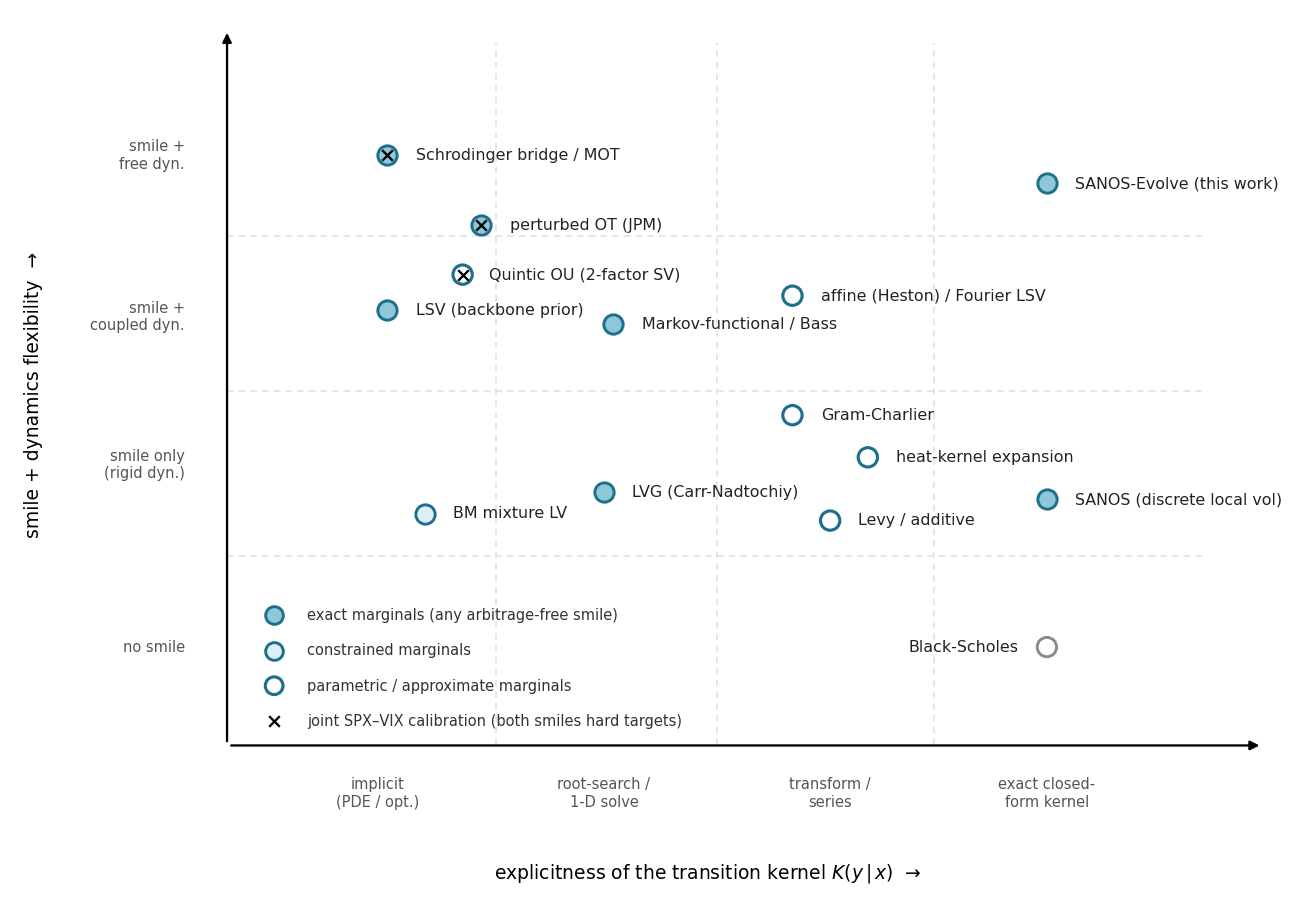
\includegraphics[width=0.72\textwidth]{figs/kernel_landscape.png}
\caption{\textbf{The transition-kernel landscape.} Explicitness of the one-step kernel $K(y\mid x)$
(horizontal), smile-and-dynamics freedom (vertical), exactness of the marginal fit (fill); tiers and
legend on the plot (Black--Scholes: no smile, fit n/a, grey). In the rightmost column, SANOS-Evolve
replaces SANOS's rigid canonical coupling with a free-dynamics Gaussian-mixture kernel
(Appendix~\ref{app:density}). A black cross marks joint SPX--VIX calibration (both smiles as hard
targets)---the programme the VIX-as-readout lane of Section~\ref{sec:intro} stays out of.
\emph{Abbreviations:} MOT/OT, (martingale) optimal transport; LSV,
stochastic-local volatility; LVG, local variance gamma; BM, Brigo--Mercurio; LV, local volatility;
SV, stochastic volatility; OU, Ornstein--Uhlenbeck.}
\label{fig:landscape}
\end{figure}

\paragraph{Contributions.}
\begin{enumerate}
  \item \textbf{A discrete SLV that decouples statics from dynamics
    (Sections~\ref{sec:marginals}--\ref{sec:kernel}).} A convex LP fixes strictly arbitrage-free
    marginals; a separately fitted martingale kernel carries the dynamics, and the marginals stay
    invariant when the dynamic targets are re-tuned. Any admissible chain is free of static arbitrage,
    with existence guaranteed by convex order (Strassen~\cite{strassen1965}). There is no leverage
    fixed point and no existence cliff, unlike classical SLV.
  \item \textbf{The SSR as an exact closed-form realised covariance, free of the smile
    (Sections~\ref{sec:twoscale},~\ref{sec:ssr}).} A translation-invariant two-timescale kernel places
    the spot--vol leverage in the return innovation around fast and slow regimes. Translation
    invariance then makes the SSR an exact realised covariance of return and regime---not a
    spot-derivative or a soft penalty---and the two timescales give its term structure, fit separately
    from the smile. This is the freedom the calibrated stochastic-volatility family lacks.
  \item \textbf{Closed-form throughout, hence deterministic
    (Sections~\ref{sec:rung},~\ref{sec:ssr}).} Prices, Greeks, the variance-index smile, and the SSR
    and forward-variance readouts are all finite Black--Scholes mixtures. Hedge ratios are therefore
    reproducible and noise-free, where particle SLV carries Monte-Carlo noise and PDE SLV carries grid
    error. The vol-of-vol is identified from a variance-index (VIX) soft target rather than by jointly
    calibrating a volatility-index market.
  \item \textbf{Scheduled-event de-eventing of the spot--vol dynamics
    (Section~\ref{sec:deevent}).} A clean-flank bridge splits a scheduled event into two closed-form
    pieces: a marginal jump density, and---the part the literature leaves open---an event-conditional
    SSR that records whether volatility jumps \emph{with} the spot at the release.
\end{enumerate}

\paragraph{Related work.}
Figure~\ref{fig:landscape} places SANOS-Evolve among transition-kernel families. The closest dynamic
relative is regime switching: Jourdain and Zhou~\cite{jourdain2020} prove existence of a calibrated
regime-switching model, a special case of local-stochastic volatility in which a finite-state process,
not the spot, carries the randomness. Our latent regime is finite-state in the same spirit, but
two-timescale and calibrated to the SSR term structure. The fast/slow structure itself is standard
multi-factor stochastic volatility in the Bergomi lineage~\cite{bergomi2009}. The Quintic OU
model~\cite{abijaber2025}---the same two-OU state under a polynomial volatility map---likewise steers
the SSR separately: even its joint SPX/VIX calibration needs an SSR band penalty, independent evidence
that the smiles do not pin the SSR. Its polynomial map buys one closed-form readout, the VIX functional;
we keep the exponential map and discretise the \emph{state} (Section~\ref{sec:twoscale}), which buys the
whole kernel. That forward implied volatility needs a transition density, not merely marginals, is the
lesson of~\cite{glasserman2010forward}.

We build on martingale optimal transport~\cite{strassen1965,beiglbock2013}: we adopt its admissible-set
constraint (with Strassen existence) but replace its objective, fitting an economically structured
kernel to dynamic targets rather than extremising an exotic's price. A neural mixture-density
surrogate~\cite{vandenberg2026} reuses the same Gaussian-mixture and CDF-loss machinery for the
opposite, simulation-surrogate objective. Scheduled-event stripping, finally, is established at the
marginal level---a discrete event-variance step~\cite{dubinsky2006,gatheraljacquier2014}, or a
clean-surface-plus-jump decomposition from non-event-spanning expiries~\cite{zhong2026,alexiou2025}---but
none of it carries the event's spot--vol dynamics. That gap is what our kernel de-eventing
(Section~\ref{sec:deevent}) fills, an open extension that a full-surface ultra-short model flags without
building~\cite{bandi2026}.

\paragraph{Scope.}
SANOS-Evolve applies to any European-option underlying. The construction needs only European exercise
(so the terminal marginal is read from prices), a liquid surface, and a forward-variance readout for the
vol-of-vol. We take SPX as the worked instance, where a liquid VIX gives the sharpest readout; equity
indices follow directly, and FX, crypto, and European single names reuse the same machinery with their
own readout and SSR (Section~\ref{sec:ssr}). Throughout, we use a readout to \emph{identify} vol-of-vol,
not to jointly calibrate a volatility-index options market---the route of the perturbed-OT desk
method~\cite{che2026pot}. Generality here is structural, a property of the construction rather than an
empirical claim across asset classes: the study is SPX. The daily framework is a methods contribution
with ground-truth validation and a real-data calibration (Section~\ref{sec:experiments}); a brief
intraday/0DTE outlook closes the discussion (Section~\ref{sec:intraday}).
%The paper is a work in
%progress: the market-data study---real-marginal calibration across regimes and the SSR-consistent hedging
%replay---is reported here (Section~\ref{sec:realdata}), not in a separate work, with a broader 
%multi-moneyness hedging study still underway.

%=============================================================================
\section{The static layer: SANOS marginals as local volatility}
\label{sec:marginals}
%=============================================================================

Fix a pricing date and maturities $T_0<T_1<\cdots<T_M$ with forwards $F_j$ and
discount factors $D_j$. Work in log-moneyness $z=\log(S/F)$. SANOS fits, at each
$T_j$, an arbitrage-free density as a Gaussian mixture in $z$,
\begin{equation}
\rho_{S,T_j}(z)=\sum_{i} q_j^{i}\,\cN\!\big(z;\mu_j^i,(\sigma_j^i)^2\big),
\qquad q_j^i\ge 0,\ \sum_i q_j^i=1,
\label{eq:sanos-marg}
\end{equation}
by a linear program over the weights $q_j$ subject to hard bid--ask boxes,
forward (martingale) normalisation, and calendar constraints~\cite{buehler2026sanos}.
We denote the resulting marginal law $\mu_j=\law(S_{T_j})$. By
Breeden--Litzenberger~\cite{breeden1978},
\eqref{eq:sanos-marg} is butterfly-arbitrage-free iff $\rho_{S,T_j}\ge 0$, which holds
by construction, and the family $\{\mu_j\}$ is calendar-arbitrage-free iff it is
increasing in convex order, which the SANOS LP enforces. By
Dupire~\cite{dupire1994}, $\{\mu_j\}$ \emph{is} the local-volatility content of the
surface.

Two structural facts make the whole construction closed-form. First, in
log-coordinates every object we use is a Gaussian mixture. Second, Black--Scholes is
not a modelling assumption but a computational identity: the call price under a
single Gaussian log-return is the moment-generating function of a truncated Gaussian,
\begin{equation}
\E\big[(S-K)^+\big]
= F\,\Phi(d_1)-K\,\Phi(d_2),\qquad
d_{1,2}=\frac{\log(F/K)\pm\tfrac12\tau^2}{\tau},
\label{eq:bs-identity}
\end{equation}
with $\tau=\sigma\sqrt{T_j}$ the total volatility. The price of any claim is then a \emph{pairing} of the
marginal with its payoff; for the mixture~\eqref{eq:sanos-marg} the call is a finite
weighted sum of Black--Scholes evaluations,
\begin{equation}
C_j(K)=\big\langle\mu_j,(\cdot-K)^+\big\rangle
=\sum_i q_j^i\,\BS\!\big(F_j^i,K,\sigma_j^i\big),\qquad
F_j^i=F_j\,e^{\mu_j^i+\frac12(\sigma_j^i)^2},
\label{eq:mix-price}
\end{equation}
with no quadrature, no PDE, and no Monte Carlo, and likewise for digitals and any payoff
with a closed-form Gaussian expectation. Because call payoffs separate measures
(Breeden--Litzenberger), this pairing is a faithful coordinate for $\mu_j$: the mixture
density makes the marginal matchable, and the closed-form pairing makes it readable.

The same mixture sum gives the Greeks in closed form---each a $q$-weighted sum of component
Black--Scholes sensitivities, no bumping and no Monte-Carlo noise. With
$d_1^i=[\log(F_j^i/K)+\tfrac12(\sigma_j^i)^2]/\sigma_j^i$,
\begin{equation}
\Delta=\frac1{S}\sum_i q_j^i F_j^i\,\Phi(d_1^i),\qquad
\mathcal V=\sum_i q_j^i F_j^i\,\varphi(d_1^i),\qquad
\Gamma=\frac1{S^2}\sum_i \frac{q_j^i F_j^i\,\varphi(d_1^i)}{\sigma_j^i},
\label{eq:mix-greeks}
\end{equation}
with $\Delta,\Gamma$ in spot and $\mathcal V$ per unit total volatility ($\times\sqrt{T_j}$ for
the annualised vega); higher sensitivities follow the same way. These are the
\emph{sticky-moneyness} Greeks of the fixed marginal, computed with the smile held fixed in
moneyness ($\SSR=0$). The desk hedge delta instead rolls the smile at the calibrated
SSR---the SSR-consistent $\Delta_{\SSR}$ of~\eqref{eq:ssr-delta}.

%=============================================================================
\section{The dynamic layer: admissible transition kernels}
\label{sec:kernel}
%=============================================================================

With the marginals fixed, this section defines what may move between them. We set up the
Markov kernel on the joint spot--regime state and carve out the \emph{admissible}
set---positive, normalised, martingale, marginal-matching---on which absence of static
arbitrage is a theorem and existence is Strassen's. Every dynamic choice in the paper is
made \emph{within} this set; Section~\ref{sec:twoscale} selects the element.

\subsection{State and kernel}
The dynamic object is a Markov chain on the joint state
\begin{equation}
X_j=(Z_j,f_j,s_j),\qquad Z_j=\log(S_{T_j}/F_j),\quad
f_j\in\{1,\dots,n_{\mathsf{F}}\},\ \ s_j\in\{1,\dots,n_{\mathsf{S}}\},
\end{equation}
where $Z_j$ is log-spot and $(f_j,s_j)$ are a \emph{fast} and a \emph{slow} latent
volatility regime---\emph{both carried} across maturities, the genuine two-timescale
(Bergomi) memory. The transition over $[T_j,T_{j+1}]$ is a Gaussian-mixture kernel that
places the spot--vol leverage in the return \emph{innovation}---a within-step node
$l=1,\dots,n_{\mathsf{L}}$ correlated with the regime moves---around a \emph{fixed} stationary vol
target:
\begin{equation}
\cK\big((z,f,s),(\dd z',f',s')\big)=\sum_{l=1}^{n_{\mathsf{L}}} w_l\,
\underbrace{P_{\mathsf{F}}(f'\mid l,f)\,P_{\mathsf{S}}(s'\mid l,s)}_{\text{two carried OU factors}}\,
\cN\!\big(\dd z';\,z+d_{f,s,l},\,V_{f,s,l}\big),
\label{eq:kernel}
\end{equation}
with $\cN(\dd z';m,V)$ the Gaussian measure with mean $m$ and variance $V$.
The \emph{coefficients} on the right---the weights $w_l$, the transitions $P_{\mathsf{F}},P_{\mathsf{S}}$, the drift
$d_{f,s,l}$ and variance $V_{f,s,l}$---are functions of the regime indices alone; the spot $z$
enters \emph{only} as the additive centre of the Gaussian, so the kernel depends on $(z,z')$
solely through the return $z'-z$. It is therefore \textbf{translation-invariant in log-spot}:
shifting spot shifts the landing law by the same amount, so the conditional return law---and
hence the smile in moneyness---depends on the regime $(f,s)$ alone, not on the spot level.
This single property keeps every dynamic readout, the SSR in particular, an exact closed form
(Section~\ref{sec:ssr}), and makes propagation an exact Gaussian-mixture map
(Section~\ref{sec:twoscale}). The within-step node $l$ carries the instantaneous skew and is
renewed each step; the two regimes are carried across steps.

\paragraph{Spot marginal vs.\ lifted law.} The kernel acts on the joint state, so its
one-step law is a \emph{lifted} joint $\widehat\mu_j(\dd z,f,s)$, whereas SANOS supplies
only the spot marginal $\mu_j^Z(\dd z)=\sum_{f,s}\widehat\mu_j(\dd z,f,s)$. The first
maturity is lifted with the stationary joint regime law $\pi_{f,s}$; thereafter the joint
is carried by the propagation. The shorthand $\mu_j\cK_j=\mu_{j+1}$ denotes the match of
\emph{spot} marginals (Remark~\ref{rem:fitproject}).

\subsection{Admissibility and no static arbitrage}
\begin{definition}[Admissible kernel]
Given forward-normalised marginals $\mu_j,\mu_{j+1}$, a Markov kernel $\cK_j$ is
\emph{admissible} if
\begin{equation}
\cA_j=\Big\{\cK_j:\ \cK_j\ge 0,\ \cK_j\mathbf 1=1,\
\E[e^{Z_{j+1}}\mid X_j=x]=e^{Z_j}\ \forall x,\
\mu_j \cK_j=\mu_{j+1}\Big\}.
\label{eq:admissible}
\end{equation}
The conditions are, in order: positivity, normalisation, the (forward-normalised)
martingale property, and exact marginal propagation.
\end{definition}

\begin{theorem}[No static arbitrage]
\label{thm:noarb}
Let $\{\mu_j\}_{j=0}^M$ be probability measures on $(0,\infty)$ with
$\E_{\mu_j}[S]=F_j$ whose forward-normalised laws $\tilde\mu_j=\law(S_{T_j}/F_j)$ are
increasing in convex order, $\tilde\mu_0\cxle\tilde\mu_1\cxle\cdots\cxle\tilde\mu_M$.
If $\cK_0,\dots,\cK_{M-1}$ are admissible (each $\cK_j\in\cA_j$), then the discrete-time
process with initial law $\mu_0$ and transitions $\{\cK_j\}$ is a martingale after
discounting, has one-dimensional marginals exactly $\{\mu_j\}$, and the induced
call surface $C_j(K)=D_j\int(s-K)^+\mu_j(\dd s)$ is free of strike (butterfly) and
calendar static arbitrage. Moreover $\cA_j\neq\emptyset$ for every $j$.
\end{theorem}

\noindent A proof sketch is given in Appendix~\ref{app:proof}. The content is that the
no-arbitrage \emph{claim attaches to the admissible set}, and that the set is nonempty
precisely because SANOS delivers marginals in convex order (Strassen). SANOS's own canonical
discrete-local-volatility coupling~\cite{buehler2026sanos} is one element of $\cA_j$---the
rigid one the introduction set out to replace; the dynamic targets of
Sections~\ref{sec:rung}--\ref{sec:ssr} (SSR, VIX, forward starts) \emph{select a different,
controllable element within} $\cA_j$---they never replace the set.

\begin{remark}[Structural marginal-matching, not fit-then-project]
\label{rem:fitproject}
The translation-invariant kernel of Section~\ref{sec:twoscale} cannot match an arbitrary
prescribed marginal by itself: a pure convolution adds the same increment law at every
spot and cannot reshape the smile. Marginal-matching is restored by a deterministic
\emph{leverage overlay} $\sigma_{\mathrm{LV}}(z,T_j)$---the discrete stochastic-local-volatility
structure---chosen by Gy\"ongy's identity so the forward map lands on the SANOS target
\emph{by construction} (Section~\ref{sec:fusion}, \eqref{eq:gyongy}). There is thus
\emph{no fit-then-project}: the first three admissibility conditions are structural in the
coefficient map and the fourth (marginal-matching) is the leverage, so calibration fits
only the \emph{dynamic} (SSR) knobs while the statics come along for free.
\end{remark}

%=============================================================================
\section{The two-timescale latent-regime kernel}
\label{sec:twoscale}
%=============================================================================

This section constructs the element of $\cA_j$ we use: the two-factor Bergomi latent
variance, Gauss--Hermite-discretised into a finite regime chain driven by nine structural
knobs, with the spot--vol leverage placed in the return innovation. Three ingredients are
arranged to be exact: the per-fibre martingale lock, the Gaussian-mixture closure under
propagation, and the Gy\"ongy leverage that lands the propagated marginals on the SANOS
targets. Recompression and semigroup interpolation then complete the toolkit.

\subsection{Two carried timescales and the Gauss--Hermite discretisation}
The latent log-variance is a baseline plus two mean-reverting Ornstein--Uhlenbeck factors---a
\emph{fast} factor $X^{\mathsf{F}}$ (rate $\kappa_{\mathsf{F}}$) and a \emph{slow} factor $X^{\mathsf{S}}$ (rate $\kappa_{\mathsf{S}}$)---so
that $x_j=\bar\gamma+X^{\mathsf{F}}_j+X^{\mathsf{S}}_j$, the continuous two-factor Bergomi model. Conditional on the latent vol the one-step log-return is
Gaussian, but its mean and variance are \emph{functions of the continuous vol state}: the
kernel is then a continuous, variable-coefficient mixture of Gaussians---an integral over the
latent factors, \emph{not} a finite Gaussian mixture, and not closed form. The remedy is
quadrature. An $n$-point \textbf{Gauss--Hermite} rule represents $\cN(0,1)$ by $n$ nodes
$\zeta_l$ and weights $w_l$ reproducing the Gaussian's moments through order $2n-1$,
\begin{equation}
\E_{\cN(0,1)}[g]=\int g(\zeta)\,\frac{e^{-\zeta^2/2}}{\sqrt{2\pi}}\,\dd\zeta
   \ \approx\ \sum_{l=1}^{n} w_l\,g(\zeta_l)\qquad(\text{exact for }\deg g\le 2n-1),
\label{eq:gh}
\end{equation}
the moment-optimal finite stand-in for a Gaussian. Replacing each continuous latent quantity
by its $n$ GH nodes turns the integral into a finite sum---each node a \emph{vol
scenario}---so the kernel becomes a finite Gaussian mixture over a quadrature grid. \emph{Both}
vol factors are carried:
\begin{itemize}
  \item \textbf{Fast factor $\mathsf{F}$}---carried regime, node index $f=1,\dots,n_{\mathsf{F}}$, mean-reversion
    $\kappa_{\mathsf{F}}$ (the high, decaying short end of the SSR);
  \item \textbf{Slow factor $\mathsf{S}$}---carried regime, node index $s=1,\dots,n_{\mathsf{S}}$, mean-reversion
    $\kappa_{\mathsf{S}}$ (the sustained long-end floor);
  \item \textbf{Within-step return $\mathsf{L}$}---node index $l=1,\dots,n_{\mathsf{L}}$, \emph{renewed} each
    step, carrying the instantaneous skew and the innovation leverage.
\end{itemize}
%Throughout, a \emph{sans-serif} $\mathsf{F},\mathsf{S},\mathsf{L}$ names the factor and the matching \emph{italic}
%$f,s,l$ its running node index. 
The nodes $\{\zeta^{\mathsf{F}}_f\},\{\zeta^{\mathsf{S}}_s\},\{\zeta^{\mathsf{L}}_l\}$ and base
log-weights $\eta^{\mathsf{F}},\eta^{\mathsf{S}}$
(within-step weights $w_l=\softmax(\eta^{\mathsf{L}})$) are \emph{fixed} quadrature constants, not
parameters (fitting the base weights as an expressive residual is a design alternative we do not
use); the data fit only the nine structural knobs of the coefficient map below. The
vol-of-vols $\nu_{\mathsf{F}},\nu_{\mathsf{S}},\nu_{\mathsf{L}}$ scale the nodes, the leverages $\lambda_{\mathsf{F}},\lambda_{\mathsf{S}}$ couple
the regime moves to the realised return node $l$ (never to $z$), and $\lambda_{\mathrm{skew}}$
tilts the within-step return. The node counts are a deliberate \emph{modelling} choice, not an accuracy dial. The within-step
factor (small $\nu_{\mathsf{L}}$) is converged at $n_{\mathsf{L}}=5$, but the carried factors converge \emph{slowly}:
$V\propto e^{\nu\zeta}$ is lognormal in the node, and Gauss--Hermite, being polynomial-exact,
resolves $\E[V]$ only gradually for the larger $\nu_{\mathsf{F}},\nu_{\mathsf{S}}$. A sweep shows the ATM-vol level
still drifting at $n_{\mathsf{F}}=9,\,n_{\mathsf{S}}=7$. We therefore keep a coarse $n_{\mathsf{F}}=5,\,n_{\mathsf{S}}=3$ and let
calibration absorb the discretisation: $\bar\gamma$ and the leverages are fit \emph{at} the
grid, so the model hits its ATM and SSR targets at any node count, and refining merely re-shifts
$\bth$. The continuous limit $n_{\mathsf{F}},n_{\mathsf{S}}\to\infty$ is thus a structural relationship, not a
practical convergence claim at these counts; the counts trade resolution against parameter
identifiability (Appendix~\ref{app:ident}) and cost.

\subsection{The coefficient map}
The component coefficients are \emph{determined} by nine structural knobs
$\bth=(\bar\gamma,\nu_{\mathsf{F}},\nu_{\mathsf{S}},\nu_{\mathsf{L}},\lambda_{\mathrm{skew}},\lambda_{\mathsf{F}},\lambda_{\mathsf{S}},\allowbreak
\kappa_{\mathsf{F}},\kappa_{\mathsf{S}})$. The per-node variance and the within-step skew tilt are
\begin{align}
V_{f,s,l}&=\exp\!\big(\bar\gamma+\nu_{\mathsf{F}}\,\zeta^{\mathsf{F}}_f+\nu_{\mathsf{S}}\,\zeta^{\mathsf{S}}_s+\nu_{\mathsf{L}}\,\zeta^{\mathsf{L}}_l\big)
  \Delta_j, &&\text{(two-factor variance)},\\
\ell_{f,s,l}&=\lambda_{\mathrm{skew}}\,\zeta^{\mathsf{L}}_l\,\sqrt{V_{f,s,l}},
  &&\text{(instantaneous mean-tilt / skew)},
\end{align}
and the two carried factors evolve by leverage-coupled mean-reverting transitions whose
tilt is driven by the realised return node $l$, \emph{not} by log-spot:
\begin{align}
P_{\mathsf{F}}(f'\mid l,f)&=\softmax_{f'}\!\big(\eta^{\mathsf{F}}_{f'}+\kappa_{\mathsf{F}}\,\zeta^{\mathsf{F}}_f\zeta^{\mathsf{F}}_{f'}
  +\lambda_{\mathsf{F}}\,\zeta^{\mathsf{L}}_l\,\zeta^{\mathsf{F}}_{f'}\big),\\
P_{\mathsf{S}}(s'\mid l,s)&=\softmax_{s'}\!\big(\eta^{\mathsf{S}}_{s'}+\kappa_{\mathsf{S}}\,\zeta^{\mathsf{S}}_s\zeta^{\mathsf{S}}_{s'}
  +\lambda_{\mathsf{S}}\,\zeta^{\mathsf{L}}_l\,\zeta^{\mathsf{S}}_{s'}\big).
\end{align}
Here $\eta$ pulls to the centre (mean reversion), $\kappa$ to the current regime
(persistence / timescale), and $\lambda_{\mathsf{F}},\lambda_{\mathsf{S}}$ are the \emph{innovation}
leverages: a down move ($\zeta^{\mathsf{L}}_l$ large via $\lambda_{\mathrm{skew}}<0$) tilts the
regimes to higher vol. Because the leverage multiplies the innovation around a
\emph{fixed} stationary target, the equilibrium vol is \emph{not} a deterministic
function of spot---it is genuine stochastic volatility, and the kernel stays
translation-invariant in $z$.

\subsection{Exact per-fibre martingale normalisation}
The within-step drift is re-locked to the forward on \emph{every} fibre---the kernel's
conditional law at a fixed state $(z,f,s)$. With raw mean
$\widetilde m_{f,s,l}=-\tfrac12 V_{f,s,l}+\ell_{f,s,l}$, subtract the per-regime constant
\begin{equation}
A_{f,s}=\log\sum_l w_l\,\exp\!\big(\widetilde m_{f,s,l}+\tfrac12 V_{f,s,l}\big)
       =\log\sum_l w_l\,e^{\,\ell_{f,s,l}},\qquad
d_{f,s,l}=\widetilde m_{f,s,l}-A_{f,s},
\label{eq:mg-norm}
\end{equation}
so that $\E[e^{Z_{j+1}}\mid z,f,s]=e^{z}$ exactly. The shift is a single per-fibre
constant, \emph{independent of $z$} (the within-step weights $w_l$ are the fixed
Gauss--Hermite weights)---stable, differentiable, and it preserves the relative branch
tilts that carry the leverage and the SSR. It replaces any penalty-only enforcement and
the fragile ``adjust one component mean'' construction, which fails when the required
numerator turns non-positive. The kernel is now complete: a finite Gaussian-mixture
martingale on $(z,f,s)$.

\subsection{Spot-translation invariance and the SSR dial}
\label{sec:invariance}
With every coefficient in \eqref{eq:kernel} independent of $z$ (Section~\ref{sec:kernel}), the
conditional smile $\sigma(T;f,s)$ depends only on the regime pair, and the skew-stickiness
ratio is generated by the \emph{innovation} leverage
$\lambda_{\mathsf{F}},\lambda_{\mathsf{S}}$ (the return$\leftrightarrow$regime correlation), not by any
$z$-coupling: $\lambda_{\mathsf{F}}=\lambda_{\mathsf{S}}=0\Rightarrow$ no spot--vol comovement
$\Rightarrow\SSR=0$ (sticky-moneyness); the dials and their term-structure shaping are
developed in Section~\ref{sec:ssr}. The SSR is
thus not a spot-derivative of a state-dependent smile but the closed-form
return$\,\times\,$regime covariance of Section~\ref{sec:ssr}. The placement of the leverage is
a design decision with teeth. A Monte-Carlo cross-check showed that coupling the regimes to
\emph{spot} instead makes the equilibrium vol a deterministic function of spot (local
volatility), which pins $\SSR\to2$ at long maturities and cannot be re-tuned. Placing the
leverage in the innovation breaks that floor while keeping the readouts exact.

\subsection{Exact Gaussian-mixture closure}
The point of translation invariance is that one propagation step is an \emph{exact Gaussian
convolution}: the finite mixture of Section~\ref{sec:twoscale} stays a finite mixture, so every
downstream readout is a closed-form sum rather than a quadrature. Conditional on the regime, the
kernel adds an increment $\Delta z\sim\cN(d_{f,s,l},V_{f,s,l})$ to the log-price
(Section~\ref{sec:invariance}), and Gaussians convolve in closed form---means and variances
add:
\begin{equation}
\cN(\,\cdot\,;m^{f,s}_c,v^{f,s}_c)\ \ast\ \cN(\,\cdot\,;d_{f,s,l},V_{f,s,l})
\ =\ \cN\!\big(\,\cdot\,;\,m^{f,s}_c+d_{f,s,l},\ v^{f,s}_c+V_{f,s,l}\big).
\label{eq:gauss-conv}
\end{equation}
So a law carried, per regime $(f,s)$, as a Gaussian mixture in log-price
$\sum_c\omega^{f,s}_c\,\cN(m^{f,s}_c,v^{f,s}_c)$ propagates to another finite mixture,
\begin{equation}
\rho_{j+1}(z',f',s')=\sum_{f,s,\,c}\omega^{f,s}_c\sum_{l}w_l\,
P_{\mathsf{F}}(f'\!\mid\! l,f)\,P_{\mathsf{S}}(s'\!\mid\! l,s)\,
\cN\!\big(z';\,m^{f,s}_c+d_{f,s,l},\,v^{f,s}_c+V_{f,s,l}\big),
\label{eq:gm-closure}
\end{equation}
each new component the convolved Gaussian of~\eqref{eq:gauss-conv}, reweighted by the within-step
weight $w_l$ and the regime transitions: $\mathrm{GM}\ast\mathrm{GM}=\mathrm{GM}$,
exactly---no quadrature, PDE, or Monte Carlo anywhere in the chain. (A \emph{state-dependent}
kernel---$z$-dependent weights $w_l(z)$ or variances---breaks~\eqref{eq:gauss-conv}: propagation
relapses to a continuous integral mixture, forcing a first-order collocation that a Monte-Carlo
cross-check showed biases the multi-step SSR.) The lone cost is that~\eqref{eq:gm-closure}
multiplies the component count by $n_{\mathsf{L}}n_{\mathsf{F}}n_{\mathsf{S}}$ each step; the
recompression of \S\ref{sec:recompress} below holds it to a fixed budget by a moment-preserving,
martingale-relocked reduction. Convex-order / calendar no-arbitrage rests on the martingale
kernel, not on this exact finite closure.

\subsection{The discrete SLV fusion: leverage carries the statics}
\label{sec:fusion}
Because the kernel is translation-invariant, $\mu_j\cK_j$ is a pure convolution---it
cannot bend its own (stochastic-vol) marginals onto a prescribed local-volatility
surface. Matching the SANOS marginals therefore needs one structural ingredient, a
deterministic leverage---exactly the stochastic-local-volatility decomposition. Split the
increment into a local scale and a unit stochastic-vol factor,
\begin{equation}
\Delta z\ \sim\ \bar d_{f,s}+\underbrace{\sigma_{\mathrm{LV}}(z,T_j)\sqrt{\Delta_j}}
  _{\text{statics (SANOS)}}\cdot\underbrace{\sqrt{\nu_{f,s}}}_{\text{SSR (kernel)}}\,\xi,
\qquad
\nu_{f,s}=\frac{\bar V_{f,s}}{\E_\pi[\bar V]},\quad
\bar V_{f,s}=\E_l[V_{f,s,l}]+\Var_l(d_{f,s,l}),
\end{equation}
where $\xi$ is a standard (unit-variance) innovation, $\bar d_{f,s}$ the per-fibre
martingale-lock drift (Section~\ref{sec:invariance}), and $\bar V_{f,s}$ the kernel's
\emph{full} one-step increment variance by the law of total variance---the within-node
$\E_l[V_{f,s,l}]$ plus the between-node mean spread $\Var_l(d_{f,s,l})$ the skew tilt
$\lambda_{\mathrm{skew}}$ creates (using $\E_l[V]$ alone mis-scales the leverage by $\sim 3\times$
at the calibrated $\lambda_{\mathrm{skew}}$). The unit factor
$\nu_{f,s}$ ($\E_\pi[\nu]=1$, with italic regime indices---not the sans-labelled vol-of-vol
amplitudes $\nu_{\mathsf F},\nu_{\mathsf S},\nu_{\mathsf L}$) keeps the kernel's
fluctuation---the regime comovement, i.e.\ the
SSR---and drops its level; $\sigma_{\mathrm{LV}}$ sets the level from the market.
Marginal-matching is then Gy\"ongy's identity~\cite{gyongy1986} in discrete form,
\begin{equation}
\sigma_{\mathrm{LV}}^2(z,T_j)=\frac{\sigma_{\mathrm{Dupire}}^2(z,T_j)}{\E[\nu\mid z]},
\label{eq:gyongy}
\end{equation}
with $\sigma_{\mathrm{Dupire}}$ from the SANOS marginals (closed-form Gaussian-mixture
call $+$ Breeden--Litzenberger density, calendar finite-difference) and $\E[\nu\mid z]$
the \emph{spot-conditional} average of the unit factor (distinct from the stationary
$\E_\pi[\nu]=1$; near $1$, tilted only by the spot--vol
correlation)---\eqref{eq:gyongy} being the exact discrete Gy\"ongy projection regardless. The decoupling is then literal: SANOS sets the statics and, through the
leverage, the local-vol roll; the kernel carries the SV response (the bulk of the SSR
level). In parameter terms the decoupling \emph{is} the split of the fused per-step variance into a
market level and a unit-mean kernel shape,
\begin{equation}
\Var\!\big(\Delta z\mid z,f,s\big)
=\underbrace{\sigma_{\mathrm{LV}}^2(z,T_j)\,\Delta_j}_{\text{level (market)}}\ \cdot\
\underbrace{\nu_{f,s}}_{\text{shape (kernel)},\ \E_\pi[\nu]=1},
\label{eq:decouple}
\end{equation}
whose $\pi$-average is exactly $\sigma_{\mathrm{LV}}^2\Delta_j$: the \emph{level} is set by the
leverage, and the kernel reaches the fused law \emph{only} through the unit-mean ratio
$\nu_{f,s}=\bar V_{f,s}/\E_\pi[\bar V]$. The kernel's own variance level is carried by
$\bar\gamma$, which multiplies every $V_{f,s,l}$ by $e^{\bar\gamma}$; this nearly divides out of
$\nu$ and is reset by $\sigma_{\mathrm{LV}}$, leaving $\bar\gamma$ nearly inert (the $\Var_l(d)$
term breaks exact $e^{\bar\gamma}$ homogeneity). What survives in $\nu$ is the
regime-\emph{relative} structure---the $\nu_{\mathsf{F}}\zeta^{\mathsf{F}}_f,
\nu_{\mathsf{S}}\zeta^{\mathsf{S}}_s$ spread of $\bar V$ and, through the transitions
$P_{\mathsf{F}},P_{\mathsf{S}}$, the leverages $\lambda_{\mathsf{F}},\lambda_{\mathsf{S}}$ and
rates $\kappa_{\mathsf{F}},\kappa_{\mathsf{S}}$---which is the SSR. (Numerically, a unit shift in
$\bar\gamma$ moves $\nu$ by $<0.2\%$, the same shift in $\nu_{\mathsf{F}}$ by tens of percent.)
In a \emph{spot-uncorrelated} state $\E[\nu\mid z]\approx1$, so the leverage barely rescales the
kernel ($\sigma_{\mathrm{LV}}\approx\sigma_{\mathrm{Dupire}}$), the smile is matched essentially
for free, and the SSR is the lone free dynamic target.

Because $\sigma_{\mathrm{LV}}(z)$ is a smooth, deterministic statics object, collocating it at
the component means affects only the level, not the SSR mechanism, which stays
translation-invariant and exact. For \emph{marginal matching}---each step re-seeded from the
target law, with regimes at their spot-uncorrelated stationary spread---the residual is then
discretisation rather than bias: the discrete Dupire under-reads the local variance at the
narrowest (short-$T$) marginals ($\sim$50--85\,bp), and this tightens with a central-difference
Dupire, finer grids, and a tail-clamped leverage. Under multi-step \emph{concatenation from a
fixed spot} (forward densities and hedging, Section~\ref{sec:recompress}) the shortcut is
\emph{not} free. The negative leverage tilt correlates high-$\nu$ regimes with low $z$, so the
spot-conditional $\E[\nu\mid z{=}0]$ falls measurably below $1$ (empirically $\approx\!0.7$ on
SPX), and approximating $\sigma_{\mathrm{LV}}\approx\sigma_{\mathrm{Dupire}}$ then \emph{under-reads}
the accumulated ATM level by of order $10\%$ in vol over a multi-month chain. There the exact
projection~\eqref{eq:gyongy} is retained: $\E[\nu\mid z]$ is negligible for reproducing marginals,
but a genuine path-conditional rescaling for absolute-level outputs such as forward implied vol
and hedge P\&L.

\subsection{Recompression: keeping the budget flat under concatenation}
\label{sec:recompress}
Recompression is a \emph{multi-step} device: a \emph{single} kernel application leaves a
manageable $n_{\mathsf{L}}n_{\mathsf{F}}n_{\mathsf{S}}$-component mixture and needs none. It is
\emph{concatenation}---composing $\cK_j\circ\cK_{j+1}\circ\cdots$ over several steps for forward
densities, exotics, or interpolation---that compounds the count: each composed step multiplies
the per-fibre spot mixture by $n_{\mathsf{L}}n_{\mathsf{F}}n_{\mathsf{S}}$ (each target fibre aggregates the $n_{\mathsf{F}}n_{\mathsf{S}}$ source regimes and the $n_{\mathsf{L}}$ within-step nodes),
so left alone the count is $(n_{\mathsf{L}}n_{\mathsf{F}}n_{\mathsf{S}})^J$ after $J$ steps. Each composed
step therefore ends with a recompression that holds the budget flat---it preserves the
\emph{propagated} marginal with fewer components; the match to the SANOS \emph{target} is the
separate Gy\"ongy step (Remark~\ref{rem:fitproject}), not part of recompression. The default is
a deterministic \emph{moment-preserving merge} (per fibre: sort by mean, split into
$n_{\mathrm{keep}}$ equal-weight chunks, match each chunk's first three moments), and one may
equivalently refit a compact martingale kernel $\widetilde\cK_j$ reproducing the propagated
marginal at the digital level,
\begin{equation}
\min_{\widetilde\cK_j}\ d_{\mathrm{CDF}}\!\big(\rho_j\widetilde\cK_j,
\rho_j\cK_j\big)
\quad\text{s.t.}\quad
\widetilde\cK_j\ge 0,\ \textstyle\sum_l\widetilde w_l\,
e^{\widetilde d_l+\frac12\widetilde\sigma_l^2}=1\ \text{(per fibre)}.
\label{eq:recompress}
\end{equation}
Because $\widetilde\cK_j$ is a martingale kernel,
$\rho_j\widetilde\cK_j\succeq_{\mathrm{cx}}\rho_j$ automatically (Strassen), so convex
order---hence calendar no-arbitrage---holds by construction and the convex-order
inequalities need not be imposed. The martingale is re-locked by~\eqref{eq:mg-norm} after the
merge (which preserves the moments of $z$ but not the forward $\E[e^z]$); a constrained
weight-LP (fixed reduced locations, weights fitted to the propagated CDF subject to exact
forward and convex order, reporting the residual) is available as a refinement where the merge
is too coarse. Recompression is done every composed step,
per-fibre (never merging away the carried regimes), deterministically, with the
residual reported.

Recompression touches only the component \emph{budget}; the marginal-match is restored
\emph{structurally}, by re-applying the Gy\"ongy leverage~\eqref{eq:gyongy} to the recompressed
mixture. The leverage is a local, deterministic rescaling read from the recompressed mixture's
own Dupire surface against the SANOS target, so it absorbs the moment-merge error in the same
operation that matches the kernel's intrinsic marginal: the per-step pipeline is
\emph{propagate} (dynamics) $\to$ \emph{recompress} (budget $+$ re-lock) $\to$ \emph{leverage}
(Gy\"ongy) $\to$ re-lock, with \emph{no projection at any step}. Convex order survives because
the match is to the convex-ordered SANOS target, and the leverage edits only the local
\emph{scale}, leaving the regime dynamics---the SSR---exact.

\subsection{Intermediate maturities: OU-semigroup interpolation}
\label{sec:interp}
Because the carried factor is OU, the generator is time-homogeneous and the transition operators form
a semigroup. Writing the latent log-variance as $x_t=g_0(t)+X^{\mathsf{F}}_t+X^{\mathsf{S}}_t$ (a
time-inhomogeneous forward-variance level $g_0$ plus a time-homogeneous generator), one interpolates
only the one-dimensional curve $g_0$ and constructs intermediate kernels by evaluation. At the midpoint
the kernel square root is the half-time semigroup element $\cK_{[T_1,T_2]}=P_{\Delta T/2}$, so
$\cK\circ\cK=P_{\Delta T}=\cK_{[T_1,T_3]}$ exactly, with no optimisation. The carried vol state is what
makes this work: the spot-only kernel (marginalising the vol state at the intermediate step) does not
compose, which is why a memoryless kernel requires a matching optimisation. Calendar no-arbitrage on
the interpolated marginal is automatic when $g_0$ gives non-decreasing total variance.

%=============================================================================
\section{The fitting step: digitals as a price metric}
\label{sec:rung}
%=============================================================================

We fit \emph{digitals} (CDFs), not prices. A digital is the strike-derivative of a
call, $-\partial_K C=1-G(K)$---one derivative above the price, one below the
density---and the bound that justifies the choice lives in the \emph{spot/strike}
variable $s$ (with $G$ the law of $S_T$):
\begin{equation}
\begin{aligned}
\sup_K|C_\bth-C_\star|
&\le\ \|C_\bth-C_\star\|_{\dot W^{1,1}}
=\int_0^\infty|G_\bth(s)-G_\star(s)|\dd s\\
&=\ W_1(\rho_\bth,\rho_\star)=\int_0^1|G_\bth^{-1}(u)-G_\star^{-1}(u)|\dd u.
\end{aligned}
\label{eq:w1}
\end{equation}

The middle equality is what makes the digital fit a \emph{price} metric: the $L^1$ norm of
$\partial_K(C_\bth-C_\star)$ is the homogeneous Sobolev $\dot W^{1,1}$ seminorm of the call-price
difference, equal to its total variation and---since $-\partial_K C$ is the digital---to the
\emph{aggregate mispricing of all digitals}. The gap $G_\star-G_\bth$ that the
band-loss~\eqref{eq:objective} drives into the bid--ask band is exactly the integrand of this
$W_1$, so fitting digitals strike by strike minimises the price-space Wasserstein distance. The
digital is the natural target because it sits one strike-derivative below the noisy density and
one above the coarse price.

\begin{remark}[Coordinate caveat]
The call payoff $(s-K)^+$ is $1$-Lipschitz in spot $s$, which is why the sup price gap
is bounded by $W_1$ in spot. In log-coordinate $z=\log s$ the integral acquires the
Jacobian weight, $\int|G_\bth-G_\star|e^z\dd z$, so an unweighted log-space CDF loss
does not by itself control call prices. Accordingly, any log-space, exponential-growth
discrepancy used adversarially below is a financial pricing discrepancy / integral
probability metric, not literally Wasserstein-$1$; we reserve ``Wasserstein'' for the
spot-coordinate bound~\eqref{eq:w1}.
\end{remark}

\paragraph{Objective.}
Collect the generator parameters $\bth$. The calibration stacks digital band-losses
over the SPX (and optional forward-start) instruments, plus the dynamic targets:
\begin{equation}
\min_\bth\ \sum_{i\in\text{SPX}}w^{\mathrm{spr}}_i\,
\mathrm{dist}\big(1-G^S_\bth(K_i),[\underline S_i,\overline S_i]\big)^2
+\beta_{\SSR}\sum_T\big(\SSR_T(\bth)-\SSR^\star_T\big)^2
+\beta_{\mathrm{vov}}\,\cR_{\mathrm{vov}}(\bth).
\label{eq:objective}
\end{equation}
Here $G^S_\bth$ is the CDF of the model's terminal law under the kernel $\bth$---the
\emph{Gy\"ongy-fused} propagated marginal, whose leverage~\eqref{eq:gyongy} carries the SANOS
statics. Writing it as the mixture $\sum_i q^i_\bth\,\cN(\,\cdot\,;\mu^i_\bth,(\sigma^i_\bth)^2)$
in log-moneyness, with component forwards $F^i_\bth=Fe^{\mu^i_\bth+\frac12(\sigma^i_\bth)^2}$,
the band-loss uses the model digital
\[
1-G^S_\bth(K_i)=\Pr{}_\bth(S>K_i)=\sum_i q^i_\bth\,\Phi(d^i_2),\qquad
d^i_2=\frac{\log(F^i_\bth/K_i)-\tfrac12(\sigma^i_\bth)^2}{\sigma^i_\bth},
\]
the Breeden--Litzenberger survival $-\partial_K C_\bth$ of the mixture call~\eqref{eq:mix-price},
fit to the market digital bid--ask band $[\underline S_i,\overline S_i]$. The $w^{\mathrm{spr}}_i$ are
inverse-spread weights and $\beta_{\SSR},\beta_{\mathrm{vov}}$ the soft-target weights;
$\SSR_T(\bth)$ is the model SSR~\eqref{eq:ssr-def} (in closed form,~\eqref{eq:ssr-model}) and
$\SSR^\star_T$ its target; $\cR_{\mathrm{vov}}(\bth)$ is the vol-of-vol readout
residual~\eqref{eq:Rvov}; both \emph{dynamic} targets---the SSR and the vol-of-vol readout---are
developed in Section~\ref{sec:ssr}. The minimisation is subject to the admissibility
constraints~\eqref{eq:admissible}. The martingale property is
one of them, enforced \emph{exactly} rather than softly: a single-marginal mixture
calibration would add a forward-matching cost
$\lambda\big(\sum_k\pi_k e^{m_k+q_k/2}-1\big)^2$ to the loss, whereas here the per-fibre
lock~\eqref{eq:mg-norm} drives the conditional forward error to zero at every state and
every~$\bth$, so the analogous term is identically zero and is dropped. Only the
genuinely free targets---marginal fit, SSR, and vol-of-vol---remain
in~\eqref{eq:objective}.

\paragraph{Two regimes for the dynamic targets.}
Where forward-start and VIX digitals are
\emph{liquid}, fit those prices directly through the band-loss and let the SSR
\emph{emerge}, validating it against the empirical value as a diagnostic---the principled,
risk-neutral route. Even then the emergent SSR is not guaranteed: the Quintic OU model fits the
full SPX \emph{and} VIX smiles jointly and still finds its SSR significantly below the market's,
restoring it with exactly such a band penalty~\cite{abijaber2025}. Where the dynamic instruments
are thin (most underlyings), the $\beta_{\SSR}$ penalty instead acts as an interpretable
\emph{steer}, its target a realized-SSR estimate or a desk view---a real-world
($\mathbb P$) quantity, not the risk-neutral SSR, so it neglects the volatility risk
premium. The penalty form is robust either way; an adversarial form (a min--max over an
exponential-growth critic for the worst-mispriced digital) is an optional alternative when
forward-start/VIX digitals are rich.

Algorithm~\ref{alg:calib} orchestrates the full daily calibration, with the SANOS LP
(Algorithm~\ref{alg:sanos}) as its static first step. The kernel fit is the one
\emph{non-convex} part---in contrast to the convex SANOS LP---and the structural
marginal-matching (Remark~\ref{rem:fitproject}: the leverage~\eqref{eq:gyongy} carries the
statics, then moment-preserving recompression re-locks the martingale) guarantees the
returned model is exactly arbitrage-free wherever the optimiser lands.

\begin{algorithm}[h]
\caption{SANOS-Evolve calibration (one pricing date).}
\label{alg:calib}
\begin{algorithmic}[1]
\Require per-maturity option chains (calls and puts) $\{(T_j,K,\text{bid/ask})\}_{j=1}^{M}$ and a discount curve (the static layer); \emph{and}---since the chains pin the marginals but not the dynamics---a dynamic anchor for the SSR/vol-of-vol: forward-starts or a vol-index (VIX for SPX) where liquid, else a realised estimate from the underlying's history. The forward curve (put--call parity) and forward-variance level (variance swap) are derived from the chains
\Ensure marginals $\{\mu_j\}$ and generator $\bth=(\bar\gamma,\nu_{\mathsf{F}},\nu_{\mathsf{S}},\nu_{\mathsf{L}},\lambda_{\mathrm{skew}},\lambda_{\mathsf{F}},\lambda_{\mathsf{S}},\kappa_{\mathsf{F}},\kappa_{\mathsf{S}})$ defining admissible kernels $\{\cK_j\}$; the desk outputs of Table~\ref{tab:desk}
\State \textbf{Static layer.} For each $T_j$, fit $\mu_j$ by the SANOS LP (Algorithm~\ref{alg:sanos}); verify increasing convex order $\mu_j\preceq_{\mathrm{cx}}\mu_{j+1}$ (the precondition of Theorem~\ref{thm:noarb}); repair the marginals if violated.
\State \textbf{Readout.} Extract the vol-of-vol level $(v_\infty,\xi_{\VIX})$ from the forward-variance readout---VIX futures and call-spreads for SPX, else the strip's variance-swap level with smile curvature and realised vol-of-vol (Table~\ref{tab:readout}); the two timescales $\kappa_{\mathsf{F}},\kappa_{\mathsf{S}}$ are \emph{both} fit, their fast/slow split resolved by the VIX vol-of-vol \emph{term structure} (the damping $D(\tau)$ at two horizons) on top of the SSR slope (Appendix~\ref{app:ident}).
\State \textbf{Regime scaffold.} Fix Gauss--Hermite nodes $\{\zeta^{\mathsf{F}}_f\},\{\zeta^{\mathsf{S}}_s\},\{\zeta^{\mathsf{L}}_l\}$ and base log-weights $\eta$; initialise $\bth$ from a global vol-quantile split and the readout.
\For{$j=1,\dots,M-1$ (warm-started across maturities)}
  \Repeat
    \State \textbf{Kernel fit.} Minimise the objective~\eqref{eq:objective} over $\bth$: digital band-loss to $\mu_{j+1}$, plus $\beta_{\SSR}$ (SSR term structure) and $\beta_{\mathrm{vov}}$ (vol-of-vol readout), subject to admissibility~\eqref{eq:admissible} (positivity, normalisation, exact martingale lock). \Comment{non-convex}
    \State \textbf{Structural match $+$ recompress.} The leverage~\eqref{eq:gyongy} lands the forward map on $\mu_{j+1}$ by construction; moment-preserving recompression (Sec.~\ref{sec:recompress}) holds the component budget and re-locks the martingale. Record the residual $d(\mu_j\cK_j,\mu_{j+1})$.
  \Until{marginal, SSR, and vol-of-vol residuals are within their bands}
\EndFor
\State \Return $\{\mu_j\},\,\bth,\,\{\cK_j\}$; price vanillas/exotics, Greeks, SSR-deltas, and de-event smiles in closed form (Table~\ref{tab:desk}).
\end{algorithmic}
\end{algorithm}

\paragraph{What lands on the desk.}
The kernel is an internal engine behind a standard vol-surface API; the desk receives the
deliverables of Table~\ref{tab:desk}, all closed-form and all functionals of the \emph{same}
calibrated object the algorithm returns. Continuously monitored barriers are the one
caveat---they need sub-stepping or a bridge correction---while the other exotics are direct
kernel functionals.

\begin{table}[h]
\centering\small
\setlength{\tabcolsep}{5pt}
\caption{What lands on the desk: every output is a functional of one calibrated object (SANOS marginals $+$ the transition kernel).}
\label{tab:desk}
\begin{tabular}{ll}
\toprule
Deliverable & Source \\
\midrule
SPX vanilla surface $+$ Greeks & spot marginals (drop-in) \\
Forward-vol surface $\widehat\Sigma^{\mathrm{fwd}}(z,k)$ & transition kernel \\
VIX-identified vol-of-vol & kernel (VIX-informed, Sec.~\ref{sec:ssr}) \\
Exotics: forward-starts, cliquets, autocallables, barriers & propagate through the kernel \\
SSR-consistent $\Delta$, vanna & kernel dynamics (Sec.~\ref{sec:ssr}) \\
De-event smile, event-jump density, event-conditional hedge & clean-flank bridge (Sec.~\ref{sec:deevent}) \\
\bottomrule
\end{tabular}
\end{table}

%=============================================================================
\section{Smile dynamics: the SSR and the forward-variance readout}
\label{sec:ssr}
%=============================================================================

This section develops the two \emph{dynamic} targets of the calibration
objective~\eqref{eq:objective}: the skew-stickiness ratio $\SSR_T(\bth)$ (the regime
comovement, in closed form below) and the forward-variance / vol-of-vol readout
$\cR_{\mathrm{vov}}(\bth)$---each a closed-form function of the generator $\bth$. The
desk-facing ATM features and the SSR-consistent hedge follow from the same machinery.

\subsection{The skew-stickiness ratio}
With $k=\log(K/F)$, ATM skew $\mathcal S_T=\partial_k\widehat\sigma_T(k)|_{k=0}$, the
SSR of Bergomi~\cite{bergomi2009} is
\begin{equation}
\SSR_T=\frac{1}{\mathcal S_T}\frac{\dd \widehat\sigma_{\mathrm{ATM},T}}{\dd\log S}.
\label{eq:ssr-def}
\end{equation}
In this convention $\SSR=1$ is \emph{sticky-strike} (fixed-strike vols pinned; the ATM
vol slides along the skew) and $\SSR=0$ is \emph{sticky-delta} (the smile rides with
spot; ATM vol unchanged). The empirical SPX term structure of Section~\ref{sec:intro} sits at
or beyond sticky-strike, never near sticky-delta. We fix this convention throughout.

\subsection{The SSR is a closed-form realised covariance}
A single marginal pins $\law(S_T)$ but not how the smile moves; that information lives in
the kernel. Because the kernel is translation-invariant in $z$
(Section~\ref{sec:invariance}), the conditional smile $\sigma(T;f,s)$ depends only on the
regime pair, so the empirical SSR---the regression of ATM-vol changes on returns---is
\emph{not} a spot-derivative but a finite closed-form sum over the regime transitions. With
$\pi_{f,s}$ the stationary law of the carried chain, $r$ the one-step return with node
values $d_{f,s,l}$, and $\mathrm{skew}(T)=\sum_{f,s}\pi_{f,s}\,\mathcal S_T(f,s)$ ($\mathcal S_T(f,s)=\partial_k\sigma(T;f,s)|_{k=0}$ the regime-conditional ATM skew),
\begin{equation}
\begin{aligned}
\SSR(T)&=\frac{\Cov\big(\Delta\sigma_{\mathrm{ATM}}(T),\,r\big)}{\Var(r)\,\mathrm{skew}(T)},\\
\Cov&=\sum_{f,s}\pi_{f,s}\sum_l w_l\,d_{f,s,l}\!\!\sum_{f',s'}\!P_{\mathsf{F}}(f'|l,f)P_{\mathsf{S}}(s'|l,s)\,
\big[\sigma(T;f',s')-\sigma(T;f,s)\big],\\
\Var(r)&=\sum_{f,s}\pi_{f,s}\Big[\sum_l w_l(d_{f,s,l}^2+V_{f,s,l})-\big(\sum_l w_l d_{f,s,l}\big)^2\Big],
\end{aligned}
\label{eq:ssr-model}
\end{equation}
with $\sigma(T;f,s)$ the ATM vol of the $(T/\Delta_j)$-step propagation started in regime $(f,s)$ ($\Var(r)$ the $\pi$-averaged conditional return variance; the between-regime mean term $\Var_\pi(\sum_l w_l d_{f,s,l})\sim0.2\%$ is higher-order and dropped). The covariance \emph{is} the leverage: a down-return
node $l$ tilts $P_{\mathsf{F}},P_{\mathsf{S}}$ toward higher vol (via $\lambda_{\mathsf{F}},\lambda_{\mathsf{S}}$), so $\Delta\sigma$
correlates with $r$. It is a finite sum over $(l,f,s,f',s')$---no spot-bump, no Monte Carlo,
no measure-transport approximation---and is Monte-Carlo-confirmed: the sum sits at the centre
of a direct one-step regression, $|\mathrm{diff}|\approx 0.005$ at 1m/3m/6m/1y
(Section~\ref{sec:synth}). Once the \eqref{eq:gyongy} leverage is in, the realised SSR picks
up a second, additive piece: a \emph{local-vol roll} $\partial_z\hat\sigma$ (the spot-shift
derivative $\dd\hat\sigma_{\mathrm{ATM}}/\dd\log S$, $z=\log(S/F)$) set by the forward-variance
curve, which is statics owned by SANOS. This sits on top of the stochastic-vol response, which
carries the bulk of the level. Both pieces are closed form, and the fused readout is likewise
Monte-Carlo-validated.

\subsection{The SSR dials}
The innovation leverages $\lambda_{\mathsf{F}},\lambda_{\mathsf{S}}$ carry the comovement (Section~\ref{sec:invariance}):
$\lambda_{\mathsf{F}}=\lambda_{\mathsf{S}}=0\Rightarrow\SSR=0$, and raising them lifts it through the sticky-strike value $\SSR=1$
toward the short-maturity diffusive limit near $2$, so the empirical SPX range
$\SSR\in[1,2]$ is a leverage-magnitude statement. Acting through the two timescales with
$\kappa_{\mathsf{F}},\kappa_{\mathsf{S}}$, they shape
the SSR \emph{term structure}---level \emph{and} slope: the fast $\kappa_{\mathsf{F}}$ gives the high,
decaying short end, the slow $\kappa_{\mathsf{S}}$ the sustained long-end floor that one factor cannot.
That is what Section~\ref{sec:rung} fits to SPX. (The SSR is regime- and vol-of-vol-dependent
rather than fixed by the variance-curve slope; a rising forward-variance curve lifts its
\emph{level} relative to a flat one~\cite{frizgatheral2024}---a leading-order, qualitative
effect, not a slope law.) Where forward-start prices are liquid, the same $(\lambda,\kappa)$ are
pinned by fitting those prices directly. The kernel prices forward-starting calls in closed form,
$C^{\mathrm{FS}}_{T_1,T_2}(k)=D_{T_2}\int\rho_{T_1}(\dd x)\int\cK_{T_1,T_2}(x,\dd y)(e^{y-x}-k)^+$,
and its strike-derivative is the forward-return survival function---the clean traded proxy for the
SSR---so the SSR \emph{emerges} as a diagnostic. How much the SSR can move at \emph{fixed} smile is
bounded: this is the decoupling band of Section~\ref{sec:synth}, the soft direction of
Appendix~\ref{app:ident} made quantitative.

\subsection{Closed-form ATM features and the SSR}
\label{sec:atm-closedform}
Because the conditional forward-return law is a Gaussian (log-normal) mixture, the ATM
implied-vol Taylor coefficients---level $\hat\sigma(0)$, skew $\hat\sigma'(0)$, curvature
$\hat\sigma''(0)$---are closed form \emph{with no Black--Scholes inversion}, by two routes.

\emph{Exact: implicit differentiation.} The implied vol solves
$C_{\mathrm{mix}}(m)=C_{\mathrm{BS}}(m,\hat\sigma(m))$ in log-moneyness $m=\log(F/K)$ (so $\partial_m=-\partial_k$ for the §\ref{sec:ssr} skew variable $k$; sign in App.~\ref{app:glide}). The level is a
single probit of the closed-form ATM mixture price, and the higher coefficients follow by
implicitly differentiating that identity (derived in full in Appendix~\ref{app:glide}),
working in the \emph{total} volatility $u=\hat\sigma\sqrt{T_j}$ (the variable the Black greeks below are taken in),
\begin{equation}
\begin{aligned}
u'(0)&=\frac{\partial_m C_{\mathrm{mix}}-\partial_m C_{\mathrm{BS}}}{\mathcal V},
\qquad
u''(0)=\frac{\partial_m^2 C_{\mathrm{mix}}-\partial_m^2 C_{\mathrm{BS}}
-2\,\mathcal V_x\,u'(0)-\mathcal V_u\,u'(0)^2}{\mathcal V},\\
\hat\sigma^{(k)}(0)&=\frac{u^{(k)}(0)}{\sqrt{T_j}},
\end{aligned}
\label{eq:iv-implicit}
\end{equation}
with the \emph{total-vol} Black--Scholes greeks vega~$\mathcal V$, vanna~$\mathcal V_x$, and volga~$\mathcal V_u$ ($u$-derivatives of $C_{\mathrm{BS}}$) and
$\partial_m^k C_{\mathrm{mix}}$ the closed-form strike-derivatives of the mixture price; the last identity annualises each coefficient. These
are exact (numerically confirmed against the bisection-inverted IV in App.~\ref{app:glide}); the SSR $\SSR=\partial_z\hat\sigma(0)/\hat\sigma'(0)$ matches the closed-form
realised covariance~\eqref{eq:ssr-model} to four decimals. We take \eqref{eq:iv-implicit} as the calibration
targets.

\emph{Leading order: cumulants.} A coarser but interpretable route reads the coefficients off
the regime-conditional mixture cumulants $\kappa_n=\partial_t^n L(0)$ of the
cumulant-generating function
\begin{equation}
L(t)=\log\sum_{l} w_l\,e^{t\,d_{f,s,l}+\frac12 t^2 V_{f,s,l}},
\label{eq:cgf}
\end{equation}
via the Gram--Charlier map $u_0=\sqrt{\kappa_2}$, $u_1=\kappa_3/6\kappa_2^{3/2}$,
$u_2=\kappa_4/12\kappa_2^{5/2}$~\cite{corradosu1996,gatheral2006}. By the law of total
cumulance $\kappa_3=\mu_3(d)+3\operatorname{Cov}(d,V)$, the skew's leverage term
$\operatorname{Cov}(d,V)$ is explicit and the Appendix~\ref{app:ident} Jacobian is analytic;
the SSR itself is the realised covariance~\eqref{eq:ssr-model}, not a spot-derivative of
these regime-conditional cumulants. The cost is accuracy---this proxy sits $8$--$9\%$ below
the exact level (skew $16$--$20\%$)---so the cumulants serve interpretation and
identifiability, not the fit.

\emph{Roughness consistency, and the SSR as a calibration map.} The inverted $\bth$ should
respect the static-to-dynamic relation $\SSR\to H+\tfrac32$ when the skew decays as
$\tau^{H-1/2}$~\cite{doeffkamal2012}, with $H$ the Hurst exponent of the volatility
process~\cite{frizgatheral2024,fukasawa2026}. Read backwards this is a calibration
rule: the SSR is the trusted observable, so an observed short-$T$ value fixes the model's
skew-dynamics exponent ($H=\SSR^\star-\tfrac32$) rather than leaving it free. The diffusive
two-OU kernel sits at $H=\tfrac12$ ($\SSR\to2$); a market $\SSR\approx 1.5$ reads as
$H\approx 0$---the roughness a multi-factor extension must hit, a derived target, not a knob.

\subsection{The SSR-consistent hedge ratio}
The desk-facing payoff is the hedge. The true delta of a strike-$K$ option carries a
smile-response term, and for a \emph{fixed} strike the sensitivity is
\begin{equation}
\Delta_{\SSR}=\Delta_{\BS}+\mathrm{Vega}\cdot\partial_S\widehat\sigma(K),\qquad
\partial_S\widehat\sigma(K)=\frac{\mathcal S_T\,(\SSR_T-1)}{S},
\label{eq:ssr-delta}
\end{equation}
where $\mathcal S_T=\partial_k\widehat\sigma$ is the ATM skew. The factor $(\SSR_T-1)$
combines the SSR's at-the-money response,
$\partial_S\widehat\sigma_{\mathrm{ATM}}=\SSR_T\,\mathcal S_T/S$, with the fixed-strike
smile-roll $-\mathcal S_T/S$. Hence sticky-strike ($\SSR=1$) gives
$\partial_S\widehat\sigma(K)=0$ and recovers the Black delta, while sticky-delta
($\SSR=0$) gives $-\mathcal S_T/S$. A Black/sticky-strike hedge omits the $(\SSR_T-1)$
term and bleeds systematic P\&L whenever the realised SSR departs from $1$---materially so
for SPX at short tenors---while the calibrated kernel supplies the adjustment its
calibrated SSR implies. We name this delta \emph{SSR-consistent} rather than
``correct'': \eqref{eq:ssr-delta} is the analytically correct hedge \emph{for a smile
rolling at the calibrated SSR}. Whether it lowers realised hedging variance against the
Black and sticky-strike deltas is a separate, empirical claim. The historical replay of
Section~\ref{sec:experiments} finds $27$--$47\%$ below Black at the money, with the broader
multi-moneyness study outstanding.

\paragraph{The hedging error.} What \eqref{eq:ssr-delta} buys is the residual it removes. For a
Black-delta hedge ($\Delta=\Delta_{\BS}$) of a strike-$K$ option, the step P\&L decomposes as
\begin{equation}
\dd V-\Delta_{\BS}\,\dd S=\underbrace{\mathrm{Vega}\cdot\frac{\mathcal S_T(\SSR_T-1)}{S}\,\dd S}_{\text{smile-roll (first order)}}
+\underbrace{\tfrac12\Gamma(\dd S)^2-\Theta\,\dd t}_{\text{gamma--theta}}+\cdots,
\label{eq:hedge-pnl}
\end{equation}
the smile-roll term being the value change from the smile moving with spot
($\dd\widehat\sigma(K)=\partial_S\widehat\sigma(K)\,\dd S$). It is a \emph{first-order} exposure,
systematic whenever $\SSR_T\ne1$, that inflates the hedging-error variance over many rebalances; the
SSR-consistent delta~\eqref{eq:ssr-delta} folds it into the spot hedge, leaving the usual
gamma--theta. The companion vanna---the spot--vol cross-greek, equally closed-form---hedges the
second-order cross: under the SSR the realised spot--vol comovement is $\SSR_T\,\mathcal S_T(\dd S)^2/S$,
an exposure the calibrated SSR likewise pins.

\subsection{The forward-variance readout (VIX as the SPX instance)}
The vol-of-vol is \emph{identified} from a readout of the underlying's forward-variance
distribution, and enters the fit only as a soft target. Its \emph{level} is the variance-swap
rate---a model-free integral of the underlying's own option strip, hence available for
\emph{any} European-option underlying with no separate product---while its \emph{dispersion}
(vol-of-vol and skew) is what a volatility-index options market prices directly; for SPX that
market is VIX, the sharpest instance. For SPX, $\VIX_T^2$ is $30$-day forward variance,
$Y_T:=\VIX_T^2=\tfrac1\tau\E_T\!\big[\int_T^{T+\tau}v_u\dd u\big]$ with $\tau\approx 30/365$,
a functional of the latent vol state. A factor with rate $\kappa$ is damped over the readout
horizon by $D(\kappa)=(1-e^{-\kappa\tau})/(\kappa\tau)$; the fast factor is strongly damped
and the slow factor barely, so the readout is slow-dominated while short-dated smile curvature
is fast-dominated. With $V^{\mathsf F},V^{\mathsf S}$ the fast/slow factor contributions to the
forward variance---affine readout $Y_T=v_\infty+D_{\mathsf F}V^{\mathsf F}+D_{\mathsf S}V^{\mathsf S}$,
$D_{\mathsf F}=D(\kappa_{\mathsf F})$, $D_{\mathsf S}=D(\kappa_{\mathsf S})$---this separates the timescales:
\begin{equation}
\Var(Y_T)=D_{\mathsf F}^2\Var(V^{\mathsf F})+D_{\mathsf S}^2\Var(V^{\mathsf S})+2D_{\mathsf F}D_{\mathsf S}\Cov(V^{\mathsf F},V^{\mathsf S}).
\label{eq:vix-var}
\end{equation}

\begin{remark}[Identification caveat]
The clean ``two observables, two unknowns'' reading---smile curvature and readout width
recover $\Var(V^{\mathsf F}),\Var(V^{\mathsf S})$---holds only once the factor correlation $\chi_{fs}$ is
fixed. Our default $\chi_{fs}=1$ pins the covariance term
in~\eqref{eq:vix-var} to $\sqrt{\Var(V^{\mathsf F})\Var(V^{\mathsf S})}$, keeping two unknowns; with
$\chi_{fs}$ free there is a third.
\end{remark}

In the discrete kernel the forward variance is regime-determined---$\VIX_T=\sqrt{\bar v_k}$
on regime $k$ with probability $p_k$---so the variance-index law is atomic and its calls are
regime sums,
\begin{equation}
C^{\VIX}(K)=e^{-rT}\sum_k p_k\big(\sqrt{\bar v_k}-K\big)^+,
\label{eq:vix-atomic}
\end{equation}
with $\bar v_k$ the forward variance carried by regime $k$: no PDE, no Monte Carlo.

\begin{remark}[Atomic vs.\ dense regimes, and the VIX smile]
\label{rem:atomic}
The VIX law in~\eqref{eq:vix-atomic} is atomic because $\VIX_T=\sqrt{\bar v_k}$ is a
deterministic function of the discrete regime; hence the VIX call is piecewise-linear
in $K$ and the VIX digital is a step function. This is harmless under our scope, where
VIX only \emph{identifies} the regime dispersion, and the atomic sum is a quadrature for
that dispersion whose accuracy improves with the regime count (a discretisation, not a
parameter, knob: the generator stays $\sim\!6$-dimensional). If a smooth VIX smile is
required, give each regime a within-regime lognormal spread,
whereupon~\eqref{eq:vix-atomic} becomes a mixture of Black calls---at the cost of one
vol-of-VIX parameter per regime.
\end{remark}

The readout enters the objective~\eqref{eq:objective} through a soft target on the kernel's
implied vol-of-vol, computed from the closed-form regime sums~\eqref{eq:vix-atomic}:
\begin{equation}
\cR_{\mathrm{vov}}(\bth)=\big(v_\infty(\bth)-v_\infty^\star\big)^2
+\sum_n\big(\xi_{\mathrm{model}}(\tau_n;\bth)-\xi_{\VIX}(\tau_n)\big)^2,
\label{eq:Rvov}
\end{equation}
the squared mismatch of the model's forward-variance \emph{level} $v_\infty$ and \emph{vol-of-vol}
$\xi$ to the readout, summed over the horizons $\{\tau_n\}$ (whose term structure pins $\kappa_{\mathsf{S}}$
through the damping $D(\tau)$; a vol-of-vol-skew term is added where a vol-index smile is liquid). It is
\emph{not} a hard marginal: we impose only \emph{unconditional} forward-variance consistency,
$\sum_k p_k y_k=\mathrm{FV}$, which is necessary but not sufficient for full joint
consistency---the conditional identity $y\approx\E[L_\tau\mid S,Y]$ that the joint
problem~\cite{guyon2022} requires is exactly what reading rather than jointly fitting forgoes.

\subsection{Extracting the readout, and what stands in for VIX}
The targets $\xi_{\VIX}$ and $\kappa_{\mathsf{S}}$ are read by a small, robust estimator rather than a
full smile fit, since the readout is a soft target. For SPX the instruments are VIX:
\begin{enumerate}
  \item \textbf{Instruments.} VIX \emph{futures} for the forward-variance level, and
    VIX \emph{call-spreads}---not pure digitals, as the model variance-index law is atomic
    (Remark~\ref{rem:atomic})---for the smile width and skew, across the listed
    maturities $\{\tau_n\}$.
  \item \textbf{Filtering.} Retain quotes inside liquid bid--ask bands and weight each
    by inverse spread.
  \item \textbf{Targets.} Futures $\to$ level / long-run variance $v_\infty$; smile
    \emph{width} $\to$ vol-of-vol $\xi_{\VIX}$; smile \emph{skew} $\to$
    vol-of-vol skew; \emph{term structure} of the width across $\{\tau_n\}$ $\to$ the
    slow rate $\kappa_{\mathsf{S}}$ via the damping $D(\tau)$.
  \item \textbf{Map to the generator.} Fix the two timescales $\kappa_{\mathsf{F}},\kappa_{\mathsf{S}}$ from the term structure of
    $\xi_{\VIX}(\tau_n)$ through $D(\tau)$ at two horizons; split $\nu_{\mathsf{S}},\nu_{\mathsf{F}}$ from
    $\xi_{\VIX}$ and the short-dated smile curvature
    via~\eqref{eq:vix-var}, conditional on $\chi_{fs}$. All enter
    $\cR_{\mathrm{vov}}$ as soft targets.
\end{enumerate}

For an underlying \emph{without} a liquid volatility-index options market the same recipe runs
against whatever readout exists, at graded identification strength (Table~\ref{tab:readout}):
the target is never empty, merely sharper for SPX. Off-SPX the readout is \emph{weakly}
identified rather than absent: the own-strip skew and
curvature give $\rho$ and $\xi$ separately but \emph{fuzzily} (the soft pair of
Appendix~\ref{app:ident}), still risk-neutral but noisy. A realised estimate optionally
firms it up, at the cost of mixing in a real-world ($\mathbb P$) quantity. VIX simply makes
the same $\mathbb Q$ separation sharp---the honest cost of generality. The vol-of-vol \emph{skew} (the upward VIX-smile slope) is third-order for the
SSR and near-ATM dynamics and has no off-SPX market source, so the parsimonious kernel omits
it; it is fitted only for VIX-pricing or deep-wing work, where SPX's liquid VIX makes it
available.

\begin{table}[h]
\centering\small
\setlength{\tabcolsep}{6pt}
\begin{tabular}{@{}lll@{}}
\toprule
Underlying & Forward-variance readout & Strength \\
\midrule
SPX & VIX futures $+$ options & sharpest (market-pinned) \\
SX5E & VSTOXX futures $+$ options & strong \\
Crypto (BTC/ETH) & DVOL index $+$ smile $+$ realised & good \\
NDX, NKY, KOSPI, HSI & vol-index level $+$ smile curvature $+$ realised & workable \\
FX (EURUSD, \dots) & risk-reversal/butterfly $+$ forward-vol & workable \\
European single names & smile curvature $+$ realised $+$ event structure & weakest \\
\midrule
\emph{any} European underlying & own-strip level $+$ smile curvature $+$ realised & universal fallback \\
\bottomrule
\end{tabular}
\caption{The forward-variance readout that identifies the kernel's vol-of-vol, by underlying.
The \emph{level} is always recoverable from the option strip; only the \emph{dispersion}
(vol-of-vol) varies in identification strength. VIX is the sharpest available instance, not a
precondition.}
\label{tab:readout}
\end{table}

The CBOE VIX is the log-contract, equal to forward variance only without jumps; a
diffusive Gaussian-mixture satisfies this, while a jump component needs the standard
convexity correction.

%=============================================================================
\section{Scheduled-event de-eventing}
\label{sec:deevent}
%=============================================================================

Section~\ref{sec:interp} interpolates \emph{within} a time-homogeneous block. Scheduled
events---FOMC and CPI for an index, earnings for a single name---are the block
\emph{boundaries}: a known date $t_k$ at which extra variance arrives and breaks the smooth
forward-variance level $g_0$ of Section~\ref{sec:interp}. The total Black--Scholes variance to
maturity carries a calendar step,
\begin{equation}
w(T)=w^{\mathrm{diff}}(T)+\!\!\sum_{t_k\le T}\!\!J_k,
\label{eq:deevent-split}
\end{equation}
a smooth diffusive curve plus a sum of event lumps $J_k$ (the saw-tooth in the ATM
total-variance term structure). The homogeneous kernel cannot absorb a lump: its per-step
conditional variance is $O(\Delta)$ while $J_k$ is an $O(1)$ point mass in calendar time---this
\emph{is} the time-homogeneity break. De-eventing strips the lumps so the homogeneous generator
$\bth$ calibrates on the clean windows, with the event a thin separate layer; left in, a flexible
surface silently absorbs the event premium and the term-structure interpolation can turn
calendar-arbitrageable~\cite{zhong2026,gatheraljacquier2014}.

Two things must be recovered, and the established methods recover only one. Every event-vol
construction---a scalar variance bump, a dirty-to-clean surface split, an additive jump
density~\cite{dubinsky2006,zhong2026}---models the event \emph{marginal}: the before-to-after
return distribution at one horizon. None records whether the volatility surface jumps \emph{with}
the spot at the release---the event's spot--vol \emph{dynamics}, an event-conditional
skew-stickiness ratio. A marginal cannot carry it (it does not pin the response,
Theorem~\ref{thm:noarb}), so a surface-plus-jump object has nowhere to hold it; a transition kernel
does. De-eventing here therefore returns \emph{both} halves---the jump density \emph{and} its
spot--vol leverage---and the second, the dynamics, is the part the literature leaves open.

\subsection{The clean-flank bridge}
Bracket the event window $[T_2,T_3]$ (the one window spanning $t_k$) by event-free windows
$[T_1,T_2]$ and $[T_3,T_4]$---the \emph{clean flanks} that name the method. The marginals
$\mu_1,\dots,\mu_4$ are read from the chains; on the
clean flanks the kernel is the homogeneous diffusive kernel
$\cK_{12}=\cK_{34}=\cK_{\mathrm{diff}}(\bth)$, so $\bth$ is identified \emph{where there is no
event}. Time-homogeneity then fixes the middle window's diffusive counterfactual---propagate the
pre-event marginal through the clean generator,
\begin{equation}
\mu_3^{\mathrm{diff}}=\cK_{\mathrm{diff}}(\bth)\,\mu_2,
\qquad
\cK^{\mathrm{obs}}_{23}=\cK_{\mathrm{diff}}(\bth)\ast\rho_J,
\label{eq:deevent-bridge}
\end{equation}
with $\rho_J$ the event-jump law and $\ast$ convolution in log-return. The event is the gap
$\mu_3\ominus\mu_3^{\mathrm{diff}}$. A pair of marginals alone does not pin the middle kernel;
the bridge closes it with two ingredients held fixed---$\bth$ from the clean flanks, and a
low-cumulant parametric ansatz for $\rho_J$.

\subsection{Two channels}
The event splits along the same statics/dynamics seam as the model.

\paragraph{Statics: the jump density.} Take $\rho_J$ \emph{additive}---independent of the
diffusive state---so \eqref{eq:deevent-bridge} is a genuine convolution and cumulants add. The
jump cumulants are then the exact residual of the observed and de-evented marginals,
\begin{equation}
\kappa_n(\rho_J)=\kappa_n(\mu_3)-\kappa_n(\mu_3^{\mathrm{diff}}),\qquad n\ge 2,
\label{eq:deevent-cumulant}
\end{equation}
recovered by a parametric (small-mixture) deconvolution at the digital level---well-posed exactly
because $\rho_J$ is low-dimensional, where a non-parametric deconvolution would not be. The second
cumulant returns the desk's scalar event variance; the third and fourth carry the event crash-skew
and the relief/sell-off bimodality. Writing
$\rho_J=\sum_m\pi^J_m\,\mathcal N\!\big(\mu^J_m,(\sigma^J_m)^2\big)$ with
$\sum_m\pi^J_m e^{\mu^J_m+\frac12(\sigma^J_m)^2}=1$ keeps the de-evented and re-evented surfaces in
closed-form finite-mixture class.

\paragraph{Dynamics: the event leverage.} The marginal $\mu_3$ does not record whether the event
jump is \emph{correlated} with the volatility move---a joint spot--vol property, the
event-conditional analogue of the SSR. It is read not from $\mu_3$ but from the forward-start smile
across $[T_2,T_3]$: the realised covariance~\eqref{eq:ssr-model} evaluated on the event transition,
the post-event ATM response $\sigma(\cdot;f',s')-\sigma(\cdot;f,s)$ weighted by the event-step
leverage $\lambda_{\mathsf{F}},\lambda_{\mathsf{S}}$.

\subsection{Hedging through the event}
An event is a known-time jump, and a delta hedge cannot catch a jump; event risk is therefore an
\emph{options} hedge, with a delta correction from the leverage, and the two channels supply both.
The static jump sizes the \emph{gamma} leg: its variance is the second cumulant $J=\kappa_2(\rho_J)$,
an implied one-event move $\sqrt J$ that the bridge separates from the diffusive variance and that
sizes the event straddle, while $\kappa_3,\kappa_4$ set the directional tilt---risk-reversals or
strangles positioned at the legs of $\rho_J$. The dynamics supply the \emph{delta} leg: the spot
hedge to hold \emph{through} the release is the SSR-consistent delta~\eqref{eq:ssr-delta} evaluated
with the event-conditional SSR,
\begin{equation}
\Delta^{\mathrm{ev}}_{\SSR}=\Delta_{\BS}+\mathrm{Vega}\cdot\frac{\mathcal S_T\,(\SSR^{\mathrm{ev}}-1)}{S},
\qquad
\SSR^{\mathrm{ev}}=\frac{\Cov(\Delta\sigma_{\mathrm{ATM}},r)}{\Var(r)\,\mathrm{skew}}\bigg|_{[T_2,T_3]},
\label{eq:event-delta}
\end{equation}
the realised covariance~\eqref{eq:ssr-model} taken on the event transition rather than the
stationary chain, with vanna the event spot--vol cross-hedge; a Black/sticky-strike hedge sets
$\SSR^{\mathrm{ev}}=1$ and bleeds the $(\SSR^{\mathrm{ev}}-1)$ term across the release. Holding that
delta through the date, the residual attributes cleanly,
\begin{equation}
\Delta\Pi\;\approx\;\underbrace{\tfrac12\Gamma(\Delta S)^2-\Theta\,\Delta t}_{\text{diffusion}}
\;+\;\underbrace{\mathrm{Vega}\cdot\Delta\sigma_{\mathrm{ev}}}_{\text{jump }(\kappa_2)}
\;+\;\underbrace{\mathrm{Vanna}\cdot\Delta S\,\Delta\sigma_{\mathrm{ev}}}_{\text{leverage }(\SSR^{\mathrm{ev}})},
\label{eq:event-pnl}
\end{equation}
into a diffusive roll, the event jump, and the leverage cross-term---the event-localized form of the
hedging error~\eqref{eq:hedge-pnl}. So the desk receives, per event,
the de-evented and re-evented surfaces with the premium isolated, the implied scenario $\rho_J$, the
gamma and event-delta legs, one coherent surface across the date, and the
attribution~\eqref{eq:event-pnl}. The first two are standard desk de-eventing; the event-conditional
delta and the leverage term are what the transition kernel adds over a surface-plus-jump object.

The split is honest about where the value sits. For index macro events, whose priced jump is
variance with little directional skew~\cite{zhong2026}, the hedge is dominated by the gamma leg and
the event-conditional delta correction is small unless the leverage is non-trivial (the empirical
question of Section~\ref{sec:deevent-synth}); for single-name earnings, whose asymmetry is
priced~\cite{alexiou2025}, the directional and event-conditional-delta legs carry more weight.

\subsection{Localised Gy\"ongy, and what is and is not new}
The bridge is the Gy\"ongy fusion~\eqref{eq:gyongy} localised to the event date: the same marginal
match, the overlay a calendar lump rather than the full local-volatility surface. Interpolation and
de-eventing are one homogeneity property read two ways---the semigroup composes \emph{within} an
event-free block (Section~\ref{sec:interp}), the lump $J_k$ is the \emph{between-block} residual it
cannot bridge. Relative to the established static de-eventing cited at the head of this section,
what \eqref{eq:deevent-bridge} supplies is the dynamics: an event-conditional SSR that the
unconditional-SSR literature does not measure. A full-surface ultra-short model that removes FOMC
days notes this accommodation ``could be \dots\ but is beyond the objectives of the current
paper''~\cite{bandi2026}. Algorithm~\ref{alg:deevent} collects the clean fit, the
counterfactual, and the two channels into one pass.

\begin{algorithm}[h]
\caption{Scheduled-event de-eventing (one event $t_k$).}
\label{alg:deevent}
\begin{algorithmic}[1]
\Require marginals on windows bracketing $t_k$: event-free flanks $[T_1,T_2],[T_3,T_4]$ and the event-spanning window $[T_2,T_3]$; the event calendar
\Ensure the diffusive generator $\bth$, the de-evented smile $\mu_3^{\mathrm{diff}}$, the event-jump density $\rho_J$, and the event leverage
\State \textbf{Clean fit.} Calibrate $\bth$ on the event-free flanks only (Algorithm~\ref{alg:calib} restricted to $[T_1,T_2],[T_3,T_4]$); the event-spanning window is held out.
\State \textbf{Counterfactual.} Propagate $\mu_3^{\mathrm{diff}}=\cK_{\mathrm{diff}}(\bth)\,\mu_2$, the de-evented prediction at $T_3$.
\State \textbf{Statics.} Form the cumulant residual~\eqref{eq:deevent-cumulant} and fit a small martingale-normalised mixture $\rho_J$ (parametric deconvolution); the de-event smile is $\mu_3^{\mathrm{diff}}$, the re-evented smile $\mu_3^{\mathrm{diff}}\ast\rho_J$.
\State \textbf{Dynamics.} Evaluate the event-conditional SSR~\eqref{eq:ssr-model} on the $[T_2,T_3]$ transition from the forward-start smile; record the event leverage.
\State \Return $\bth,\ \mu_3^{\mathrm{diff}},\ \rho_J,\ \text{event leverage}$.
\end{algorithmic}
\end{algorithm}

%=============================================================================
\section{Empirical study: ground-truth validation and real-data calibration}
\label{sec:experiments}
%=============================================================================

The study has two halves. On synthetic ground truth---where the generator is known---we verify
what the market cannot: that the closed forms are exact, that the statics/dynamics decoupling is a
genuine bounded degree of freedom, and that the de-eventing estimators recover planted truth
(Sections~\ref{sec:synth},~\ref{sec:deevent-synth}). The real-data study is the application: real
SANOS marginals, the SSR$+$vov fit across regimes, the off-SPX (NDX) generalisation, and the
SSR-consistent hedging replay (Section~\ref{sec:realdata}).

\subsection{Ground-truth validation on synthetic data}
\label{sec:synth}
All checks run at a fixed reference generator $\bth_0$ (nine knobs, calibrated once to canonical SPX
term-structure targets; values in Figure~\ref{fig:synth}), on a synthetic arbitrage-free chain where
every quantity is computable both in closed form and by simulation.

\begin{figure}[htbp]
\centering
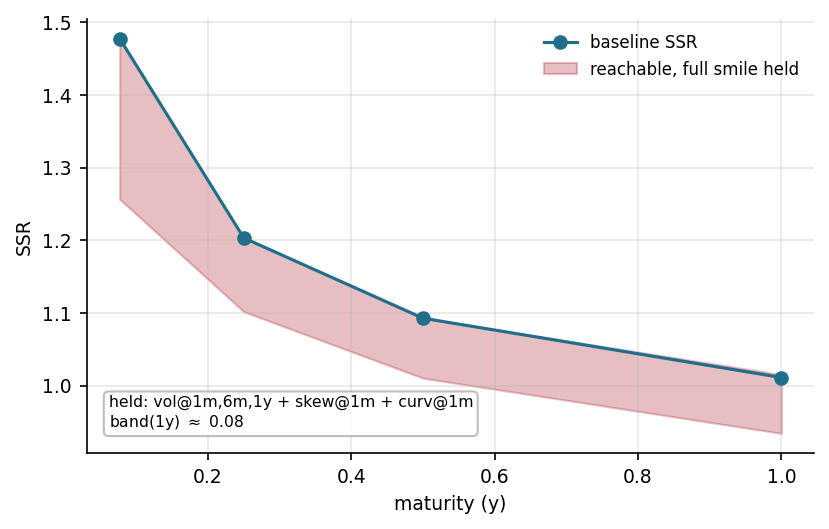
\includegraphics[width=0.62\textwidth]{figs/synthetic_main.png}
\caption{The statics/dynamics decoupling band at the reference generator (closed form, $n_k=20$).
Moving along the steepest \emph{static-preserving} direction---the null-space of the static Jacobian
holding \emph{five} smile observables (ATM vol at 1m/6m/1y; skew and curvature at 1m), Newton-held to
$\lesssim 1$\,bp in the vols and $10^{-3}$ in skew---the SSR is freely movable only inside the shaded
band: the long end spans $\approx 0.93$--$1.02$ (width $0.08$) at \emph{fixed}
statics. $\bth_0=(\bar\gamma\,{-}5.30,\nu_{\mathsf{F}}\,0.43,\nu_{\mathsf{S}}\,0.50,\nu_{\mathsf{L}}\,0.14,
\lambda_{\mathrm{skew}}\,{-}1.48,\lambda_{\mathsf{F}}\,0.98,\lambda_{\mathsf{S}}\,1.65,\kappa_{\mathsf{F}}\,1.00,
\kappa_{\mathsf{S}}\,2.34)$.}
\label{fig:synth}
\end{figure}

\paragraph{Decoupling and identifiability.} The dynamics are a genuine but \emph{narrow} degree of
freedom over the statics. Along the steepest static-preserving direction (the null-space of the
static Jacobian holding the five smile observables of Figure~\ref{fig:synth}), the SSR(1y) is freely
movable only inside a width-$\mathbf{0.08}$ band $[0.93,1.02]$ at \emph{fixed} statics. Relaxing the
hold to the three-observable smile (ATM vol at 1m/1y, 1m skew) roughly doubles the reach
($\approx[0.89,1.07]$), which contains the market long-end SSR (${\approx}1.05$). The freedom is
non-zero (genuine SV, off the local-vol floor) and bounded---wider moves recruit the statics, which the
full calibration supplies.
The elasticity-scaled Jacobian has effective rank ${\approx}7$; the closed-form
VIX vol-of-vol pins the \emph{timescale} half of the soft direction (a $12\times$
regularisation), leaving the slow leverage $\lambda_{\mathsf{S}}$ for forward-start skew
(Appendix~\ref{app:ident}).

\paragraph{Exactness (Monte-Carlo)---the anchor.} The closed-form realised SSR sits within Monte-Carlo
noise of a direct simulation ($|\mathrm{diff}|\approx0.005$ at 1m--1y; the fused SLV SSR $\le0.007$), and
the check has teeth---an earlier source-averaged form was off by $0.105$ on a skewed target, which the
Monte Carlo caught. The dynamic readouts are exact closed forms, not approximations, and this is what the
real-data residuals are read against. With the machinery proven exact here, the regime-dependence and
two-factor ceiling on real chains (Section~\ref{sec:realdata}) are properties of the data and the model's
scope, not numerical error.

\paragraph{Scope at the short end.} The kernel is diffusive ($H{=}\tfrac12$), so the model SSR rises
toward the short-end limit $2$; matching SPX's rough sub-month level (${\approx}1.5$) needs a rough
multi-factor extension ($\SSR\to H+\tfrac32$~\cite{fukasawa2026}).

\subsection{Scheduled-event de-eventing: synthetic validation}
\label{sec:deevent-synth}
We validate both channels of Section~\ref{sec:deevent} on the reference generator $\bth_0$, closed form.

\paragraph{The dynamics channel is non-redundant.} Inject an event that bumps only the regime-transition
leverage $(\lambda_{\mathsf{F}},\lambda_{\mathsf{S}})$, leaving the within-step return $(d,V)$ untouched.
Because $\lambda_{\mathsf{F}},\lambda_{\mathsf{S}}$ enter only the transitions, which integrate out of the
one-step spot marginal, the event-horizon marginal is \emph{exactly} unchanged
($|\Delta\mathrm{var}|=|\Delta\mathrm{skew}|=0$ to machine precision) while the forward-start SSR moves
monotonically with the injected leverage (Figure~\ref{fig:deevent-nr}). The event leverage is thus
identifiable, yet \emph{provably invisible} to any static de-eventing. It is the non-redundant degree of
freedom the dynamics channel adds over the static literature, and it is what licenses reading the
real-data SSR \emph{suppression} (Section~\ref{sec:realdata}: the same curve, on its leverage-down side)
as a genuine dynamics signal rather than a static-variance artifact. A symmetric martingale variance jump, meanwhile,
reproduces the index-macro ``variance, not skew'' fact~\cite{zhong2026} and leaves this leverage signal
intact.

\begin{figure}[htbp]
\centering
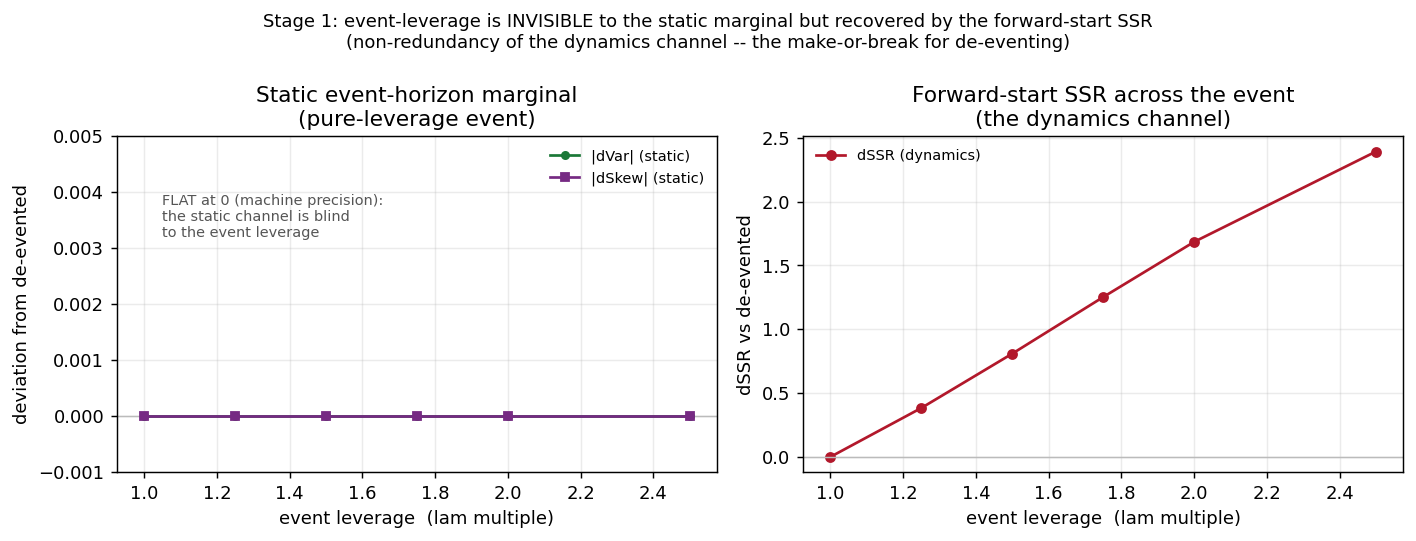
\includegraphics[width=\textwidth]{figs/deevent_nonredundancy.png}
\caption{Event-leverage non-redundancy (reference $\bth_0$, closed form). \textbf{Left:} the
static event-horizon marginal stays at machine-precision zero deviation---a pure-leverage event is
invisible to it. \textbf{Right:} the forward-start SSR across the event rises monotonically with the
event leverage. The dynamics channel carries signal the static marginal provably cannot see.}
\label{fig:deevent-nr}
\end{figure}

\paragraph{The static channel recovers a known jump.} Injecting a known asymmetric two-leg jump and
running the bridge recovers its variance, skew and kurtosis exactly (to $\sim\!10^{-16}$) and re-events the
smile to $0.00$\,bp (Figure~\ref{fig:deevent-rec})---the ground-truth check the market cannot give. Because
de-eventing is a deconvolution (jump/clean variance $0.38$ here), the recovered \emph{variance} is robust
($\pm4\%$ under $\pm2\%$ quote noise) while the \emph{skew} is noise-sensitive---itself a mechanism behind
the empirical ``variance, not skew.''

\begin{figure}[htbp]
\centering
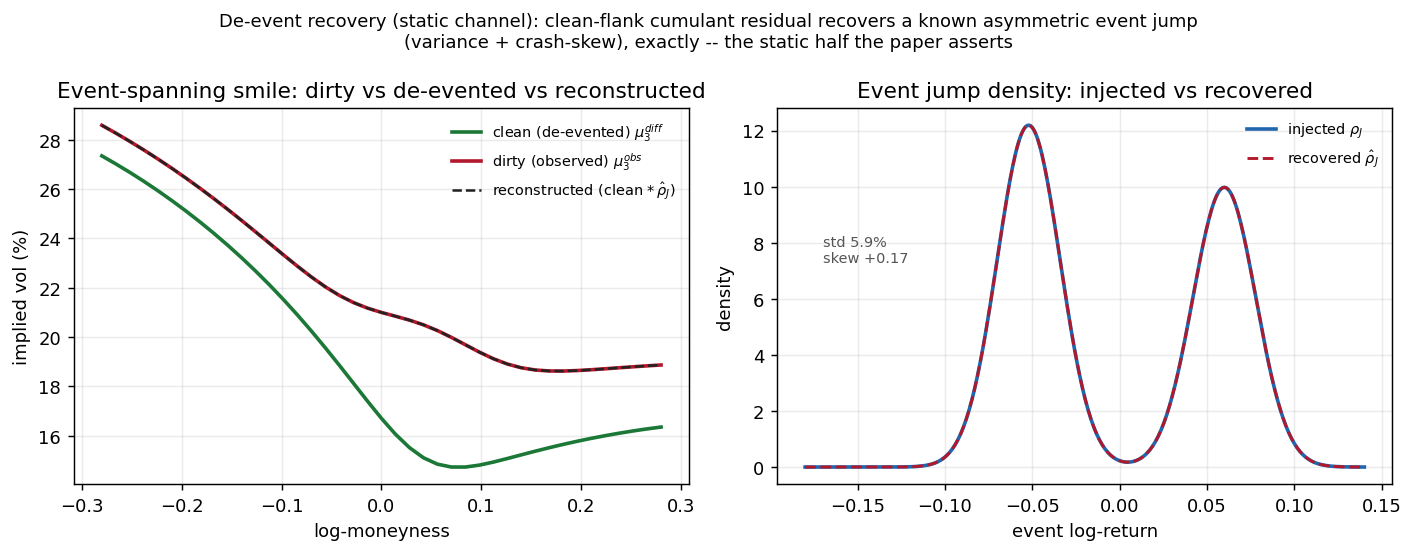
\includegraphics[width=\textwidth]{figs/deevent_recovery.png}
\caption{De-event recovery, static channel (3-month window). \textbf{Left:} the event-spanning
(dirty) smile, the de-evented (clean) counterfactual, and the reconstruction clean $\ast\,\hat\rho_J$,
which overlays the dirty smile to $0.00$\,bp. \textbf{Right:} the injected asymmetric two-leg
event-jump density and its recovery from the cumulant residual.}
\label{fig:deevent-rec}
\end{figure}

\subsection{Real-data study: results}
\label{sec:realdata}

\paragraph{SPX calibration.} On real ORATS SPX end-of-day chains the pipeline runs end-to-end.
\emph{Statics and propagation:} SANOS marginals fit across ${\sim}20$ maturities to ${\sim}2.5$\,y (convex
order holds), and one admissible kernel propagates between adjacent maturities under the exact martingale
lock~\eqref{eq:mg-norm}. The marginal-propagation residual $d(\mu_j\cK_j,\mu_{j+1})$, after the structural
Gy\"ongy match and re-seeded from each real $\mu_j$, is a median $\approx 3$ call-price bp and $\approx 26$
ATM-vol bp on the liquid surface ($\le 6$\,m), within bid--ask. It rises to $\lesssim 35$ call-bp only at the
sparse long end, where adjacent expiries are $26$--$52$ steps apart and discretisation accumulates.
\emph{Forward-start:} the forward-start return density is exact (mass and forward equal $1$ to machine
precision) and its forward skew rolls down with tenor ($\approx -0.5\!\to\!-0.14$), flatter than the spot
skew---the smile motion of Section~\ref{sec:ssr}. \emph{Dynamics:} the SSR$+$vov fit reproduces both the
realised skew-stickiness term structure~\eqref{eq:ssr-model} and the VIX vol-of-vol, at ${\le}3\%$ RMS on both
blocks for calm and moderate dates (Table~\ref{tab:realdata}, Figure~\ref{fig:real-spx}).

\begin{table}[h]
\centering
{\small
\begin{tabular}{lcc}
\toprule
Diagnostic & Result (real SPX) & Target \\
\midrule
Marginal residual $d(\mu_j\cK_j,\mu_{j+1})$ & $3$ call-bp / $26$ IV-bp ($\le$6\,m) & within bid--ask \\
SSR$_T$ fit (calm/moderate) & $0.6$--$2.3\%$ RMS & realised $1.8\!\to\!1.5$ \\
VIX vol-of-vol $\xi$ (soft target) & $1\%$ (calm)--$9\%$ (high-vol) & VIX-implied \\
Forward-smile & valid density; skew roll-down & --- \\
\bottomrule
\end{tabular}
}
\caption{Real-SPX diagnostics; the multi-start SSR$+$vov fit over 2015--2023 (autodiff
Jacobian, ridge regularisation, cached target; ${\sim}250$--$450$\,s/date on GPU).}
\label{tab:realdata}
\end{table}

\begin{figure}[htbp]
\centering
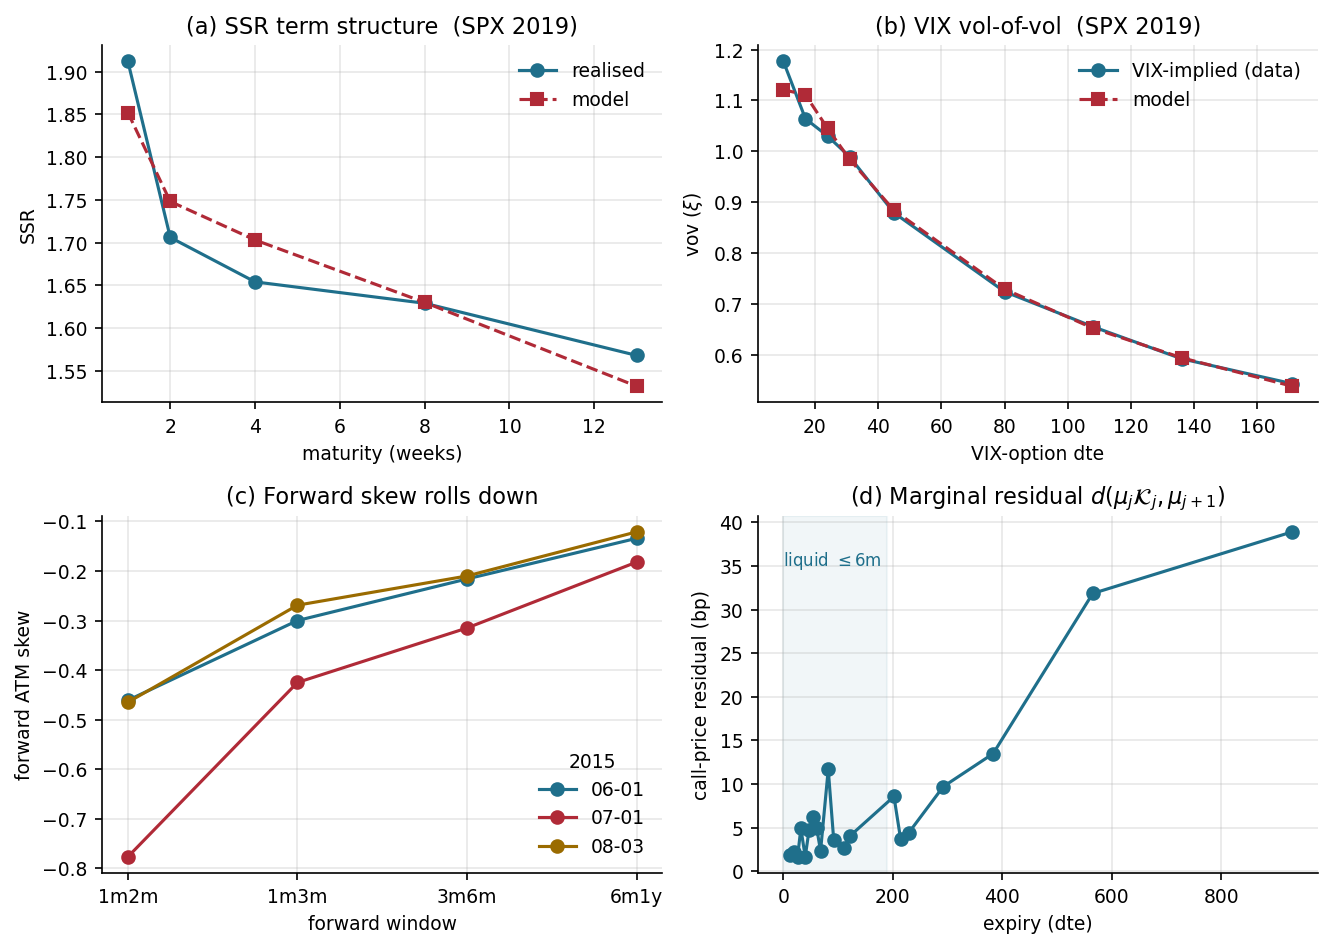
\includegraphics[width=\textwidth]{figs/real_spx.png}
\caption{Real-SPX calibration. \textbf{(a)}~The SSR$+$vov fit reproduces the realised SSR term structure (2019);
\textbf{(b)}~and the VIX vol-of-vol across VIX-option maturities. \textbf{(c)}~The forward-start ATM skew rolls
down (flattens) with tenor across dates---the smile motion of Section~\ref{sec:ssr}. \textbf{(d)}~The
marginal-propagation residual $d(\mu_j\cK_j,\mu_{j+1})$ (2015-06-01): a few call-bp on the liquid surface,
growing only at the sparse long end where adjacent expiries are many steps apart.}
\label{fig:real-spx}
\end{figure}

\paragraph{Cross-regime, and the two-factor ceiling.} Calm and moderate regimes fit to ${\le}3\%$ on both
blocks, while high-vol and post-spike dates expose the two-factor VIX vol-of-vol \emph{shape}
limit---its vol-of-vol
term structure cannot flatten at the short-mid the way those regimes priced (Table~\ref{tab:crossregime},
Figure~\ref{fig:real-offspx}a). The \emph{grind} of
2022--2023 is no exception: its realised SSR is normal (${\approx}1.25$--$1.30$), and the 2022 and 2023 SSR$+$vov
fits reach SSR RMS $3.2\%$ and $9.2\%$ (moderate). The residual sits in the VIX vol-of-vol (both
${\approx}22\%$)---the two-factor vov shape ceiling (a vov term structure the two-OU kernel cannot flatten at
the short--mid), more severe than in the 2020 high-vol regime ($9\%$), not an SSR misfit. \emph{And the
vol-of-vol target does not tax the SSR:} on the 2022 grind, a $25\times$ increase in the weight on the
vol-of-vol term leaves the SSR RMS within $2.3$--$3.2\%$, so reading the vol-of-vol off the imperfect VIX
target costs nothing on the primary SSR fit. For from-spot
outputs the exact second-order leverage~\eqref{eq:gyongy} is retained: the spot-conditional
$\E[\nu\mid z{=}0]\approx0.7$ (not $1$) lifts the accumulated from-spot ATM level by ${\sim}10\%$ in vol.

\paragraph{Off-SPX generalisation (NDX).} The model travels off SPX with \emph{own-strip and realised targets
only}, no vol-index options: NDX statics from its own SANOS marginals, the leverage from its realised SSR, and
the vol-of-vol from the realised variance-of-variance of its own model-free variance-swap strip (the graded
readout of Section~\ref{sec:ssr}; validated in that the reconstructed SPX $\sqrt V$ tracks the VIX index).
Across 2018--2022, with multi-start, NDX calibrates to $5$--$12\%$ SSR and $1$--$8\%$ vol-of-vol (bar the
$2021$ vov shape ceiling, ${\sim}19\%$)---weaker than SPX in \emph{both} blocks (its SSR RMS runs roughly
double SPX's in matched years, $2018$/$2020$), as expected from the purely physical-measure realised readout
(no vol-index, no risk-neutral target) and its ${\sim}10\%$ reconstruction bias. Cross-sectionally NDX's vol-of-vol
(${\sim}1.5$) exceeds SPX's (${\sim}1.2$)---tech is a jumpier vol process---and its marginal is modestly
fat-tailed (${\sim}2$--$3\times$ the data's excess kurtosis), a discretisation feature. The own-strip
curvature was tested as a vol-of-vol backbone and kept as a diagnostic, not a fit target
(Figure~\ref{fig:real-offspx}).

\begin{table}[h]
\centering
{\small
\begin{tabular}{llcc}
\toprule
under. & regime & SSR RMS & VIX / vov RMS \\
\midrule
SPX & 2015 calm & $0.6\%$ & $1.2\%$ \\
SPX & 2019 moderate & $2.3\%$ & $2.6\%$ \\
SPX & 2020 COVID & $3.8\%$ & $9.0\%$ \\
SPX & 2022 grind & $3.2\%$ & $22.2\%$ \\
SPX & 2023 grind & $9.2\%$ & $22.6\%$ \\
\midrule
NDX & 2018 moderate & $8.9\%$ & $4.9\%$ \\
NDX & 2021 melt-up & $5.0\%$ & $18.7\%$ \\
NDX & 2022 bear & $6.4\%$ & $1.1\%$ \\
\bottomrule
\end{tabular}
}
\caption{Fit quality across regimes and underlyings (SPX: SSR$+$vov, the vov read from VIX; NDX: SSR$+$realised
variance-of-variance, no VIX). Multi-start GPU wall-time ${\sim}250$--$450$\,s/date (SPX), ${\sim}120$--$190$\,s (NDX).}
\label{tab:crossregime}
\end{table}

\begin{figure}[htbp]
\centering
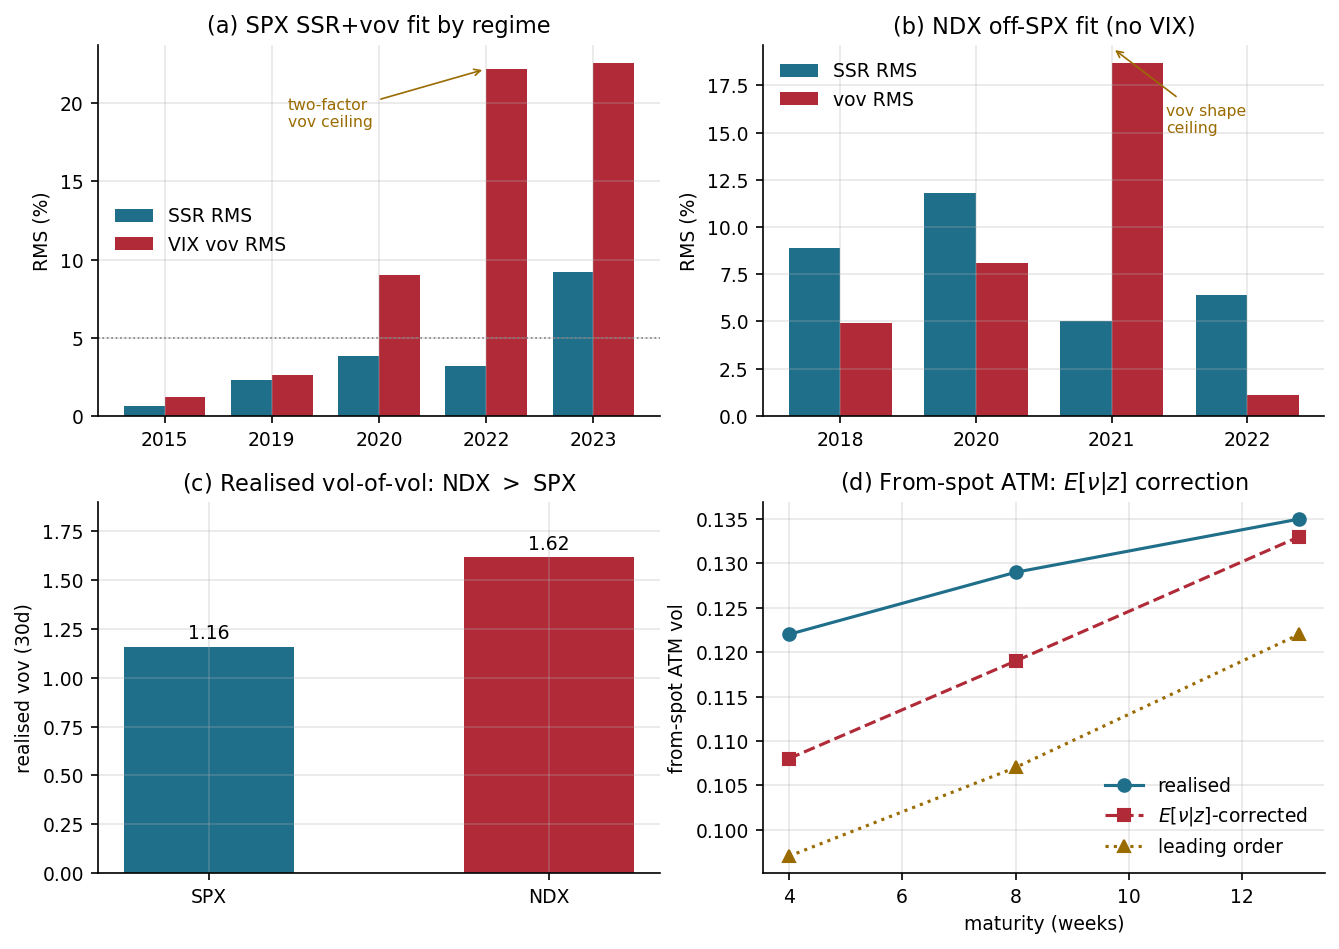
\includegraphics[width=\textwidth]{figs/real_offspx.png}
\caption{Cross-regime and off-SPX. \textbf{(a)}~SPX SSR$+$vov fit RMS by regime---calm/moderate at ${\le}3\%$,
high-vol and post-spike (incl.\ the 2023 grind) exposing the two-factor VIX vol-of-vol ceiling.
\textbf{(b)}~NDX calibrated with own-strip and realised targets \emph{only} (no VIX): $5$--$12\%$ SSR and
$1$--$8\%$ vol-of-vol except the 2021 shape ceiling (${\sim}19\%$). \textbf{(c)}~NDX's realised vol-of-vol exceeds
SPX's---tech is a jumpier vol process. \textbf{(d)}~The second-order $\E[\nu\mid z]$ leverage correction lifts
the accumulated from-spot ATM level toward the realised.}
\label{fig:real-offspx}
\end{figure}

\paragraph{Smile dynamics: the level rides, the shape sticks.}
The same exact-$\beta$ readout, taken across the whole at-the-money neighbourhood rather than at the level
alone, places the calibrated model on the sticky map (the convention of Section~\ref{sec:ssr}) in two
independent coordinates (Figure~\ref{fig:dynamics}). The \emph{level} rides with spot at the SSR,
$\partial_{\ln S}\sigma_{\mathrm{ATM}}=\SSR\,\mathcal S$, with $\SSR$ running from $2.0$ at one week down to
$1.4$ at three months: far from sticky-moneyness ($\SSR{=}0$), between sticky-strike ($1$) and the local-vol
limit ($2$), and on the Doeff--Kamal $H{+}\tfrac32$ backbone through the belly. The \emph{shape}, by contrast,
barely moves---the skew's own response $\partial_{\ln S}\mathcal S$, normalised by the rate at which a
strike-pinned smile would swing it (twice the curvature), is only $0.01$--$0.02$: the skew is essentially
\emph{frozen in moneyness} (sticky-moneyness \emph{in shape}), with a small, realistic steepening on sell-offs.
So the model reproduces the textbook equity picture---the smile \emph{shape} translates with spot while its
\emph{level} lifts on sell-offs (Figure~\ref{fig:dynamics}b: the one-month smile shifts up nearly in parallel on
a $1\%$ drop, unlike the flat sticky-moneyness or the tilted sticky-strike responses). This is also why the
SSR-consistent delta is the right hedge: with the shape sticky and only the level riding, the whole hedging
problem collapses to folding in that level move---the $\SSR$---which is exactly what~\eqref{eq:ssr-delta} does.

The frozen shape, however, is as much a \emph{structural constraint} as an empirical match. By translation
invariance (Section~\ref{sec:invariance}) the conditional smile depends on the volatility regime alone, not
on the spot level, so the shape can respond to a spot move only \emph{indirectly}---through the
leverage-induced regime shift, where a down move tilts the regime toward higher, steeper-skew vol (the small
sell-off steepening above). A \emph{deterministic, spot-level-dependent} shape---a smile intrinsically
steeper at lower index levels, beyond that stochastic-regime channel---is outside the model's reach: the same
invariance that makes the SSR an exact closed form forbids it. So where the data carry such second-order,
level-dependent skew dynamics, the ``shape sticks'' finding is a property of the construction as much as of
the market.

\begin{figure}[htbp]
\centering
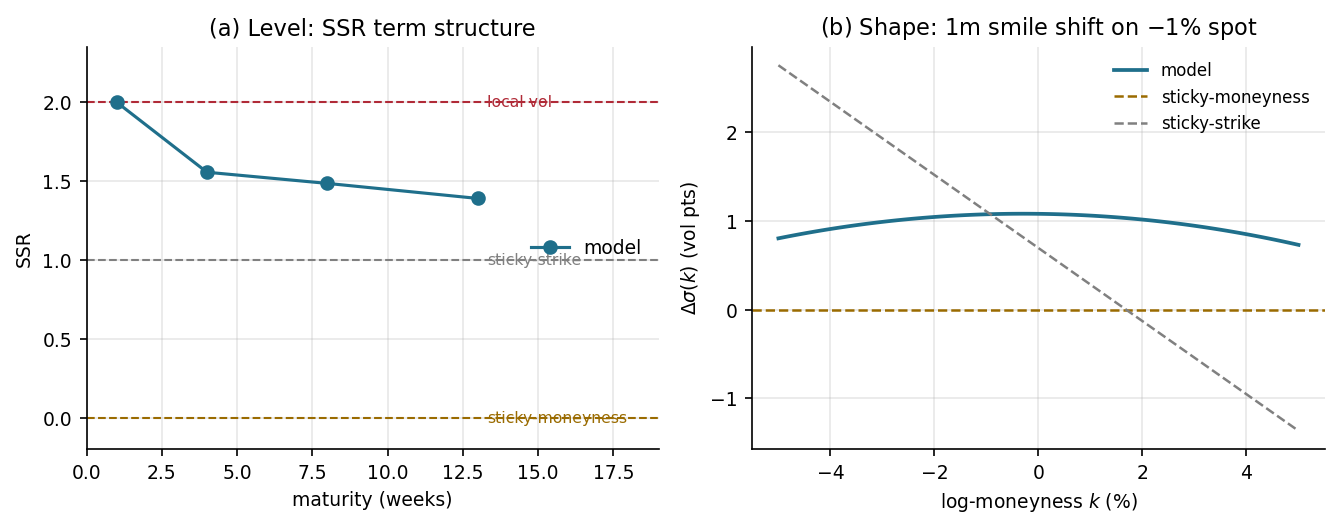
\includegraphics[width=\textwidth]{figs/real_dynamics.png}
\caption{Where the calibrated model sits on the sticky map (SPX, the exact conditional-smile response to a spot
move, decomposed by moment). \textbf{(a)}~\emph{Level}: the SSR term structure runs $2.0\!\to\!1.4$---between
sticky-strike ($1$) and local vol ($2$), far above sticky-moneyness ($0$). \textbf{(b)}~\emph{Shape}: the
one-month smile's response to a $-1\%$ spot move is a near-parallel upward shift ($\sim\!{+}1$ vol point), close
to the flat sticky-moneyness line and unlike the tilted sticky-strike one---the shape is frozen in moneyness
while the level rides.}
\label{fig:dynamics}
\end{figure}

\paragraph{Real-SPX de-eventing, statics: a symmetric variance jump.}
The clean-flank bridge recovers \emph{both} channels of Section~\ref{sec:deevent}, split along the
statics/dynamics seam. On the daily-grid era (2022--2024, $48$ FOMC$+$CPI events vs $30$ clean controls
${\ge}5$ days from any release), the counterfactual $\mu_3^{\mathrm{diff}}$ is a \emph{single} time-rescaled step
from the last clean $\mu_2$ (Alg.~\ref{alg:deevent}, step~2), taken \emph{without} recompression. A from-spot
propagation would instead cold-start the third moment---it builds skew from a point mass over many steps, each
recompression shaving it, so at the short event horizon it reads skew ${\approx}{-}0.8$ against a market
${\approx}{-}2.4$---whereas anchoring on $\mu_2$ inherits the skew directly. The event jump is then a clean
variance lump: the implied move $\sqrt J$ ($J{=}\kappa_2$ of $\rho_J$) is ${\approx}1\%$ on events vs
${\approx}0.6\%$ on controls, consistent with the term-structure lump~\eqref{eq:deevent-split}, and carries
\emph{no} directional skew. Reading the residual asymmetry at \emph{matched} variance (the lump set to the
exact $\kappa_2$ residual~\eqref{eq:deevent-cumulant}, so the two smiles share a second moment and only shape
can differ) leaves a large but \emph{event-independent} put-skew deficit: $t{\approx}8$ on events and controls
alike---the transition-side shape error of a single-step, instantaneous-Gy\"ongy counterfactual
(\S\ref{sec:fusion}, which pins marginals not the transition)---with net event-minus-control $t{\approx}{-}0.7$. That is ``variance, not skew''~\cite{zhong2026} on index macro, confirmed
and robust to the counterfactual construction.

\paragraph{Real-SPX de-eventing, dynamics: a switched-off event leverage.}
The signature the static literature cannot form is in the dynamics. For FOMC and nonfarm-payroll
releases the event-conditional SSR---the realised
$\Delta\sigma_{\mathrm{ATM}}\!\leftrightarrow\!r$ slope across the announcement
transition~\eqref{eq:event-delta}---is \emph{significantly suppressed} in normal regimes: across
2015--2019 it falls from a clean ${\approx}2.2$ to ${\approx}0.9$ at one week (FOMC
$\mathrm{dSSR}{\approx}{-}1.4$, payrolls ${\approx}{-}0.7$; pooled heteroskedasticity-robust
$t{\approx}3.7$, stable under an $|r|$-crush control)---the smile dropping from near local-vol
toward sticky-strike on the release. CPI shows \emph{no} suppression in that low-inflation era
($\mathrm{dSSR}{\approx}0$, $t{\approx}0.5$); it became the dominant macro surprise only in
2021--22, inside the grind regime below. Calibrated back into the kernel, the event bump
reproduces the suppression by driving the stochastic-vol leverage
$(\lambda_{\mathsf F},\lambda_{\mathsf S})$ to zero, and with it the SSR's stochastic-vol component
(${\approx}{+}0.4\to{\approx}0$). The event \emph{switches off} the spot--vol leverage rather than
adding skew---the kernel-native degree of freedom the marginal provably cannot carry
(Section~\ref{sec:deevent-synth}). The two halves are complementary: a symmetric
variance jump the static literature already prices, and a switched-off event leverage only the
transition kernel measures.

\paragraph{Hedging: the SSR-consistent delta.}
The ``better delta'' claim---the centrepiece---is a historical replay. We delta-hedge a rolling
one-month ATM SPX option once per day over the one-parameter family
$\Delta(R)=\Delta_{\mathrm{BS}}+\mathrm{Vega}\cdot R\,\mathcal{S}/S$~\eqref{eq:ssr-delta}, which spans the
standard deltas: $R{=}0$ is Black (sticky-strike), $R{=}-1$ is sticky-delta, and $R$ equal to the SSR is the
minimum-variance delta. The one-day hedging-P\&L variance is minimised at $R^\star$ equal to the
\emph{realised} SSR, and the SSR-consistent delta cuts it sharply below Black
(Figure~\ref{fig:hedge}, Table~\ref{tab:hedge}): across 2016--2021, $R^\star\approx1.5$--$1.8$, tracking the
realised SSR ($1.3$--$1.6$), and hedging at the model's structural $R{=}1.6$ reduces the realised hedging
variance by \textbf{27--47\%} versus Black. Sticky-delta ($R{=}-1$) is \emph{worse} than Black---it moves the
delta with the vol--spot comovement the wrong way. Two honest readings temper the headline. That a
skew-adjusted delta beats Black on an equity index is the \emph{expected} minimum-variance-delta
effect~\cite{bergomi2016,hullwhite2017}. The replay's content is its size and stability at a fixed,
option-implied $R$. And the replay does not yet isolate the model's value-add over the cheap
alternative---a trailing \emph{realised}-SSR delta, which would plausibly track $R^\star$ as well. Whether
the model's forward-looking $R$ forecasts next-period comovement better than that backward-looking
estimate is the decisive head-to-head, listed below. This edge is a \emph{normal-regime} property: it scales with
the realised SSR, so it is largest in calm/moderate markets ($\SSR\approx\tfrac32$). The reduction is out-of-sample (a fixed structural $R$, not
re-fit to each hedging window) and survives transaction costs at SPX liquidity: the vol-adjustment term raises
turnover, but by a small fraction of the variance it removes, and a smoothed model skew (in place of the raw
per-day skew used here) would cut that turnover further. \emph{Still to come:} the full study extends this across
moneyness and tenor with tail-loss and cost-curve detail, ablates the VIX layer, the two-timescale memory,
and the SSR target, and runs the real-data analogues of the Section~\ref{sec:synth} checks (the Monte-Carlo
SSR regression; the identifiability gain of Appendix~\ref{app:ident} on the real readout).

\begin{table}[htbp]
\centering{\small
\begin{tabular}{lcccc}
\toprule
year & days & realised SSR & $R^\star$ & var.\ reduction vs Black \\
\midrule
2016 & 251 & $1.42$ & $1.70$ & $45\%$ \\
2017 & 250 & $1.28$ & $1.45$ & $27\%$ \\
2019 & 251 & $1.56$ & $1.75$ & $47\%$ \\
2021 & 251 & $1.46$ & $1.60$ & $44\%$ \\
\bottomrule
\end{tabular}}
\caption{SSR-consistent hedging (one-month ATM SPX, daily rehedge). The variance-minimising delta parameter
$R^\star$ tracks the realised SSR; hedging at the model's structural $R{=}1.6$ reduces the one-day hedging
variance $27$--$47\%$ versus Black. Sticky-delta ($R{=}-1$, not shown) \emph{increases} it by $37$--$46\%$.}
\label{tab:hedge}
\end{table}

\begin{figure}[htbp]
\centering
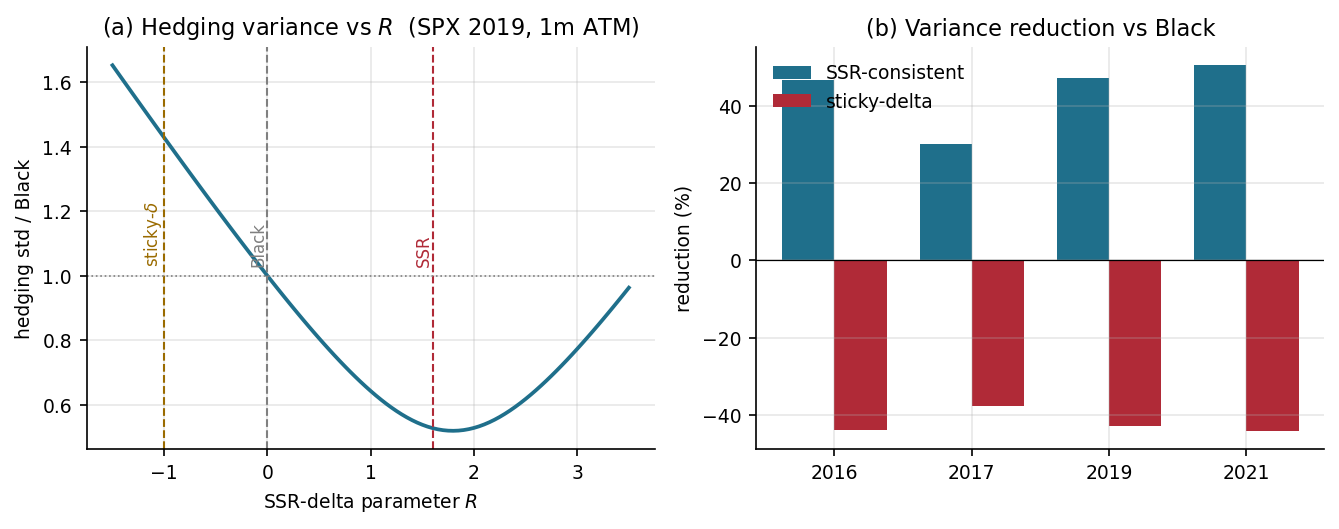
\includegraphics[width=\textwidth]{figs/real_hedge.png}
\caption{Hedging replay (one-month ATM SPX, daily rehedge). \textbf{(a)}~The one-day hedging-P\&L variance
(normalised to Black) as a function of the SSR-delta parameter $R$, for 2019: a clean U minimised near the
realised SSR and far below Black ($R{=}0$); sticky-delta ($R{=}-1$) is worse. \textbf{(b)}~The SSR-consistent
delta ($R{=}1.6$) reduces the hedging variance $27$--$47\%$ versus Black across years, while sticky-delta
increases it.}
\label{fig:hedge}
\end{figure}

\paragraph{Scope: ATM dynamics; full-smile dynamics as future work.} The statics match the full vanilla
smile, but the \emph{dynamic} layer is calibrated to \emph{at-the-money} observables---the SSR and the VIX
ATM vol-of-vol. Two full-smile extensions are left to a sequel. First, the VIX \emph{smile}---its skew and
tails, not only the ATM level---is a richer risk-neutral reading of the vol-of-vol \emph{shape}; the atomic
VIX law (Sec.~\ref{sec:ssr}) prices it across strikes with no new machinery, tightening the vol-of-vol
identification, though---being vol-of-vol---it is \emph{complementary to, not a substitute for}, the leverage
that carries the SSR. Second, the \emph{forward-start} smile skew is the clean risk-neutral observable of the
spot--vol leverage: it pins the slow leverage $\lambda_{\mathsf S}$ that vol-of-vol leaves soft
(Appendix~\ref{app:ident}) and would supersede the realised-SSR (physical-measure) proxy used here---but it
requires traded forward-start / cliquet quotes, which are over-the-counter and absent from listed-option
feeds (ORATS included), so this route is contingent on data. Together these carry the calibration from ATM- to
full-smile dynamics, of interest for cliquet and forward-volatility pricing.

%=============================================================================
\section{Discussion}
\label{sec:positioning}
%=============================================================================
With the construction and the empirical results in hand, we can be precise about what
SANOS-Evolve buys over classical SLV, which already matches vanilla marginals and produces
smile dynamics.

The differentiator, previewed in Section~\ref{sec:intro}, is the SSR. The documented rigidity
of the calibrated stochastic-volatility family~\cite{bourgey2024,frizgatheral2024} is
established for the \emph{pure} SV class, but it transfers to classical SLV: the leverage is
\emph{consumed} matching the vanilla smile, so the residual spot--vol dynamics---and hence the
SSR---falls to the stochastic-volatility backbone~\cite{bergomi2017,guyonhl2012}, and an SLV on
a standard backbone inherits the same band. SANOS-Evolve is itself a discrete SLV, so its
escape cannot come from the leverage---it comes from the \emph{backbone}: a discrete
regime-transition kernel whose two-timescale innovation leverage shapes the SSR term structure
directly while the SANOS LP holds the marginals fixed; the calibration of
Section~\ref{sec:experiments} realises this on the empirical SPX term structure.

The differences are \emph{not} approximation power---both are universal at the marginal (SLV
through a nonparametric leverage function; SANOS-Evolve through $W_1$-dense Gaussian-mixture
marginals and a sufficiently rich kernel). They are \emph{where the structure sits} and
\emph{whether the dynamics are controlled}. Classical SLV sits on the other side of each
contribution of Section~\ref{sec:intro}. Its SSR is whatever the stochastic-volatility backbone
produces, not a target. Its leverage is a fixed point of the calibration, so re-tuning the
dynamics re-triggers it, and it can fail outright when vol-of-vol is large (the leverage
$\sigma_{LV}^2=\sigma_{\mathrm{Dupire}}^2/\E[V\mid S]$ diverging), whereas the admissible set here
is never empty (Strassen, Theorem~\ref{thm:noarb}). Its Monte-Carlo particle noise (worst in the
wings, seed-dependent day to day) or PDE grid error sits inside the hedge ratios, where our
mixture pricing is deterministic. And its dynamics live in a nonparametric leverage surface,
against our nine interpretable knobs and latent regimes.

\paragraph{Universal statics, parsimonious dynamics.}
The two layers make opposite choices, on purpose. The static layer is universal: $W_1$-dense
Gaussian mixtures (Appendix~\ref{app:density}) fit \emph{any} arbitrage-free smile exactly---a
structural guarantee, not a fitted approximation---so the smile match is never the binding
constraint. The dynamic layer is parsimonious: the small propagation residual
$d(\mu_j\cK_j,\mu_{j+1})$ is a modelling choice, not a wall (a denser kernel, $W_1$-universal
too, shrinks it toward zero), and a few knobs pin the dynamics to interpretable regimes where
an unconstrained kernel would leave them underdetermined. Admissibility is exact regardless of
the residual (Remark~\ref{rem:fitproject}: the leverage carries the statics, recompression
re-locks the martingale). What lets universality and parsimony coexist is
translation-invariance: exact marginal match, few interpretable parameters, and exact
closed-form closure---jointly unsatisfiable for a \emph{state-dependent} kernel---hold together
because the translation-invariant kernel has exact Gaussian-mixture closure on the
parsimonious generator.

\paragraph{Honest costs.} The model is discrete, so continuously-monitored barriers need
sub-stepping. Recompression keeps the component budget finite (a computational cost, not an
approximation limit). The one first-order approximation is the smooth-leverage collocation on
the statics, with the dynamics staying exact by translation-invariance. And the framework is
empirically unproven relative to battle-tested SLV. Against \emph{frontier}
SLV (multi-factor, rough, or neural-SDE~\cite{cuchiero2020}), which also fit dynamics
flexibly, the edge narrows to the closed-form/deterministic/interpretable combination
rather than dynamics control per se. Three further caveats: the empirical edge is
regime-dependent---${\le}3\%$ SSR$+$vov fits in calm and moderate markets, the two-factor vol-of-vol ceiling
in stress (Table~\ref{tab:crossregime}), which is where dynamics matter most; the two-timescale split is
itself the least-identified block (Appendix~\ref{app:ident}); and the static layer rests on
SANOS~\cite{buehler2026sanos}, at this writing a preprint. Table~\ref{tab:ledger} is the precise accounting: what is
exact, what is approximate, and where each approximation sits.

\begin{table}[h]
\centering\small
\setlength{\tabcolsep}{4pt}
\renewcommand{\arraystretch}{1.15}
\begin{tabular}{>{\raggedright\arraybackslash}p{0.18\textwidth}>{\raggedright\arraybackslash}p{0.41\textwidth}>{\raggedright\arraybackslash}p{0.31\textwidth}}
\toprule
status & object & note \\
\midrule
\textbf{exact} (closed form) & the translation-invariant kernel and per-fibre lock
(\S\ref{sec:twoscale}); the realised-covariance SSR~\eqref{eq:ssr-model}; the ATM Taylor
coefficients (App.~\ref{app:glide}); the mixture cumulants; static no-arbitrage
(Thm.~\ref{thm:noarb}, Strassen) & independent of every dynamic approximation; $z$-invariance
is what makes the SSR exact, Monte-Carlo-confirmed ($|\mathrm{diff}|\!\approx\!0.005$) \\
\textbf{leverage collocation} (check first) & the smooth local-vol leverage
$\sigma_{\mathrm{LV}}(z)$ collocated at the component means (\S\ref{sec:fusion}) & moves the
statics \emph{level}, not the SSR mechanism (which stays $z$-exact); single-step benign, but a
$\sim$10\% multi-month vol-level bias if the exact $\E[\nu\mid z]$ projection~\eqref{eq:gyongy} is
dropped (\S\ref{sec:fusion}) \\
\textbf{controlled} (convergent) & recompression to $n_{\mathrm{keep}}\!\approx\!24$
(\S\ref{sec:recompress}); the discrete Dupire under-reads at narrow marginals
($\sim$50--85\,bp short-$T$) & accuracy dials---central-difference Dupire, finer grids,
tail-clamped leverage \\
\textbf{leading-order} (cross-check) & the cumulant-to-IV route
(\S\ref{sec:atm-closedform}, $\sim$8--9\% off) & \emph{not} the primary readout; the exact
coefficients (App.~\ref{app:glide}) supersede it \\
\textbf{structural limit} & short-$T$ diffusive $\SSR\!\to\!2$ ($H{=}\tfrac12$) vs SPX's rough
$\approx\!1.5$ & a modelling gap, not numerical error; fix $=$ a rough multi-factor extension \\
\textbf{structural limit} & spot-level-\emph{independent} smile \emph{shape}: the conditional smile
depends on the vol regime, not $z$ (\S\ref{sec:invariance}) & shape responds to spot only via the
stochastic-regime channel; deterministic level-dependent skew dynamics are out of reach---the flip
side of translation-invariance \\
\textbf{out of scope} & the wings / Lee moment-index regime & a finite Gaussian mixture is
structurally thin-tailed there; ATM by design \\
\bottomrule
\end{tabular}
\caption{What is exact and what is approximate. The contrast with a state-dependent
(spot-level) kernel is the point: there the quantity to check first is a measure-transport
collapse \emph{inside the dynamics}; here the only first-order approximation is a
smooth-leverage collocation \emph{on the statics}, the dynamics left exact by
translation-invariance.}
\label{tab:ledger}
\end{table}

\iffalse  % comparison table tab:slv-compare masked 2026-06-29 -- kept for possible later use
\begin{table}[t]
\centering
\small
\setlength{\tabcolsep}{6pt}
\renewcommand{\arraystretch}{1.25}
\begin{tabular}{@{}l ccccccc@{}}
\toprule
& \rotatebox{90}{Arb-free marginals\,} & \rotatebox{90}{SSR a direct target\,}
& \rotatebox{90}{Hard no-arbitrage\,} & \rotatebox{90}{Existence guaranteed\,}
& \rotatebox{90}{Noise-free Greeks\,} & \rotatebox{90}{Statics/dynamics decoupled\,}
& \rotatebox{90}{Battle-tested\,} \\
\midrule
Local volatility~\cite{dupire1994} & \checkmark & $\times$ & \checkmark & \checkmark & \checkmark & --- & \checkmark\checkmark \\
1-factor SLV (particle/PDE)~\cite{guyonhl2012,ren2007} & \checkmark & ($\checkmark$) & \checkmark & $\times$ & ($\checkmark$) & $\times$ & \checkmark\checkmark \\
Frontier SLV (rough, neural)~\cite{cuchiero2020} & \checkmark & \checkmark & ($\checkmark$) & ($\checkmark$) & ($\checkmark$) & $\times$ & ($\checkmark$) \\
SSR-targeted SV (Quintic OU)~\cite{abijaber2025} & ($\checkmark$) & \checkmark & \checkmark & \checkmark & ($\checkmark$) & $\times$ & ($\checkmark$) \\
Joint SPX--VIX~\cite{guyon2022} & \checkmark & \checkmark & \checkmark & $\times$ & $\times$ & $\times$ & ($\checkmark$) \\
\textbf{SANOS-Evolve} (this paper) & \checkmark & \checkmark & \checkmark & \checkmark & \checkmark & \checkmark & $\times$ \\
\bottomrule
\end{tabular}
\caption{Structural comparison of smile-dynamics methods. \checkmark{}~holds by
construction; ($\checkmark$)~partial or method-dependent; $\times$~absent;
---~not applicable; \checkmark\checkmark{}~extensively production-proven. The columns are
\emph{structural} guarantees of each construction, not measured performance. SANOS-Evolve
alone combines all six structural properties, but it is the only entry not yet empirically
validated---local volatility and classical SLV are battle-tested in production, which
SANOS-Evolve is not. Speed is omitted: closed-form pricing makes it plausibly fast, but
this is unbenchmarked (particle SLV is slow, PDE moderate, neural surrogates fast after
training). Citations are representative, not exhaustive.}
\label{tab:slv-compare}
\end{table}
\fi

\paragraph{Outlook: intraday and 0DTE.}\label{sec:intraday}
Same-day-expiry (``0DTE'') options are now a majority of S\&P~500 option volume, and the
construction ports there by \emph{scale invariance}. The marginal mixtures, the kernel, and
recompression and interpolation (Secs.~\ref{sec:recompress},~\ref{sec:interp}) are
clock-agnostic, so rescaling the two Ornstein--Uhlenbeck timescales---fast
$\kappa_{\mathsf{F}}$ in minutes, slow $\kappa_{\mathsf{S}}$ in hours---re-targets the model at
the 0DTE surface. Its natural dynamic target is the \emph{intraday} SSR: by the same
$D(\kappa T)$ damping that makes VIX slow-dominated, a minute/hour vol factor is averaged out
of any multi-day option and is visible only there. A genuine intraday model needs three localized
additions---a time-of-day seasonality $\phi(u)$, scheduled-event martingale jumps (the
de-eventing layer of Sec.~\ref{sec:deevent} at intraday resolution), and a terminal/pin
refinement as $T\to0$---plus synchronized intraday NBBO data; we leave the empirical 0DTE
study to a dedicated sequel.

%=============================================================================
\section{Conclusion}
\label{sec:conclusion}
%=============================================================================

SANOS-Evolve keeps the part of the option-surface problem that SANOS already solves
well---arbitrage-free marginals, the local-volatility content---and evolves it into a
stochastic-local-volatility model by fitting a martingale transition kernel with a
latent two-timescale volatility regime. The marginals stay strictly arbitrage-free, and the
kernel supplies the smile dynamics that local volatility gets wrong. The SSR is an exact
closed-form realised covariance of return and regime, and the vol-of-vol is identified---not
jointly fitted---from a forward-variance readout: VIX for SPX, but recoverable from any
European-option surface. The construction needs only European exercise, so it applies to
equity indices, FX, and crypto alike; SPX is the worked instance. Everything is closed-form,
the no-arbitrage guarantee is a theorem on an admissible set with Strassen existence, and the
desk outputs---forward densities, de-event smiles, SSR-consistent deltas---are functionals of
one object. The empirical study (Section~\ref{sec:experiments}) validates the machinery on
synthetic ground truth and reports the real-data calibration across regimes, with a hedging
replay in which the SSR-consistent delta cuts realised variance $27$--$47\%$ below Black. What
remains is the broader multi-moneyness, multi-tenor hedging study.

\appendix
%=============================================================================
\section{The SANOS marginal-calibration LP}
\label{app:sanoslp}
%=============================================================================

For completeness, Algorithm~\ref{alg:sanos} states the SANOS static-layer calibration in
this paper's notation; the original is~\cite{buehler2026sanos}. It fits, per maturity, a
weights-only Gaussian mixture whose call surface lands within bid--ask and is strictly free
of butterfly and calendar arbitrage (positivity $\to$ valid density; forward constraint
$\to$ martingale; convex-order inequality $\to$ calendar). The problem is convex---a linear
program for a piecewise-linear smoothing penalty $\mathcal R$, quadratic for a quadratic
one---and feasible within the quote bands by construction. This is the admissible-marginal
layer $\{\mu_j\}$ on which Theorem~\ref{thm:noarb} and its convex-order precondition rest.

\begin{algorithm}[h]
\caption{SANOS marginal-calibration LP at maturity $T_j$ (this paper's notation; after~\cite{buehler2026sanos}).}
\label{alg:sanos}
\begin{algorithmic}[1]
\Require strikes $\{K_{j,m}\}$ with bid/ask $[B_{j,m},A_{j,m}]$, mids $C^{\mathrm{mid}}_{j,m}$, weights $\omega_{j,m}$; forward $F_j$; fixed anchors $\{a_i\}_{i=1}^{N}$ in $z=\log(S/F_j)$; bandwidth $h$; previous-maturity fit $q_{j-1}$
\Ensure weights $q_j\ge0$ with $\rho_{S,T_j}(z)=\sum_i q_j^i\,\mathcal N(z;a_i,h^2)$, strictly arbitrage-free
\State Build the linear pricing map $(\Pi_j)_{m,i}=\BS\!\big(F_j e^{a_i+h^2/2},\,K_{j,m},\,h\big)$, the price of basis component $i$ at strike $K_{j,m}$.
\State Solve the linear program over $(q_j,t)\ge0$:
\Statex $\displaystyle\qquad \min\ \ \sum_m \omega_{j,m}\,t_m \;+\; \lambda_h\,\mathcal R(q_j)$
\Statex $\qquad \text{s.t.}\ \ -t_m \le (\Pi_j q_j)_m - C^{\mathrm{mid}}_{j,m} \le t_m \qquad (L^1\text{ fit to mids})$
\Statex $\qquad \phantom{\text{s.t.}}\ \ B_{j,m} \le (\Pi_j q_j)_m \le A_{j,m} \qquad (\text{hard bid--ask box})$
\Statex $\qquad \phantom{\text{s.t.}}\ \ \mathbf 1^\top q_j = 1,\quad \textstyle\sum_i q_j^i\,e^{a_i+h^2/2}=1 \qquad (\text{normalisation; forward})$
\Statex $\qquad \phantom{\text{s.t.}}\ \ \widehat C_j(K_g)\ge \widehat C_{j-1}(K_g)\ \ \forall K_g \text{ on a dense grid} \qquad (\text{calendar / convex order})$
\State \Return $q_j$; the CDF is $G_{S,T_j}(K)=\sum_i q_j^i\,\Phi\!\big((\log(K/F_j)-a_i)/h\big)$.
\end{algorithmic}
\end{algorithm}

%=============================================================================
\section{Proof sketch of Theorem~\ref{thm:noarb}}
\label{app:proof}
%=============================================================================

\emph{Strike no-arbitrage.} For each $j$, $\mu_j$ is a probability measure with
$\E_{\mu_j}[S]=F_j$; hence $C_j(K)=D_j\int(s-K)^+\mu_j(\dd s)$ is convex and
non-increasing in $K$ with the correct bounds, which is equivalent to absence of
butterfly arbitrage (Breeden--Litzenberger).

\emph{Martingale and marginals.} Admissibility gives $\E[e^{Z_{j+1}}\mid X_j]=e^{Z_j}$,
i.e.\ the forward-normalised price is a martingale, and $\mu_j\cK_j=\mu_{j+1}$ propagates
the law, so the chain has one-dimensional marginals exactly $\{\mu_j\}$ and the discounted
underlying is a martingale.

\emph{Calendar no-arbitrage.} A martingale transition implies, by conditional Jensen,
that the forward-normalised marginals are increasing in convex order,
$\tilde\mu_j\cxle\tilde\mu_{j+1}$, which is equivalent to absence of calendar
arbitrage for the call surface.

\emph{Existence.} By Strassen's theorem~\cite{strassen1965,beiglbock2013}, a
martingale kernel with $\mu_j\cK_j=\mu_{j+1}$ exists iff $\tilde\mu_j\cxle\tilde\mu_{j+1}$.
SANOS enforces this convex order across maturities, so $\cA_j\neq\emptyset$. \hfill$\square$

%=============================================================================
\section{Wasserstein-1 universality of Gaussian-mixture marginals and kernels}
\label{app:density}
%=============================================================================

That the mixture layer is \emph{effectively nonparametric}---the expressiveness it gives
the statics (Section~\ref{sec:intro})---rests on a denseness fact, which we make precise here
\emph{in the topology that governs option prices}. Gaussian mixtures approximate any
arbitrage-free marginal, and any continuous admissible kernel, to arbitrary accuracy, with the
approximant exactly forward-matched.

\emph{The pricing topology is $W_1$, not weak\(^*\).} Work in the spot $s=e^z$. The observables
are the undiscounted calls $\Lambda_k(\rho)=\langle\rho,(s-k)^+\rangle$, whose payoff is
$1$-Lipschitz in $s$, together with the forward $\langle\rho,s\rangle$. The coarsest topology
making all of these continuous is the Wasserstein-$1$ topology on $\mathcal P_1(\R_{+})$, the laws
of finite first spot-moment; by Kantorovich--Rubinstein and~\eqref{eq:w1},
\[
\sup_{k}\,\big|\Lambda_k(\mu)-\Lambda_k(\nu)\big|\ \le\ W_1(\mu,\nu)
=\int_0^\infty|G_\mu(s)-G_\nu(s)|\,\dd s
=\big\|C_\mu-C_\nu\big\|_{\dot W^{1,1}},
\]
the aggregate digital mispricing---\emph{exactly the band-loss the calibration minimises}
(Section~\ref{sec:rung}). Weak\(^*\) convergence is strictly too weak here: the call payoff
$(s-k)^+$ and the forward $s$ are continuous but \emph{unbounded}, hence not weak\(^*\) test
functions, so mass escaping to the tail moves prices while the marginal is held fixed against the
bounded-continuous $C_b$. Wasserstein-$1$ is precisely weak\(^*\) \emph{plus} the
uniformly-integrable first moment that pins the forward and the option values. The martingale
constraint is the single linear condition $\langle\rho,s\rangle=F$.

\begin{lemma}[Marginal universality in $W_1$]\label{lem:marg-dense}
For any arbitrage-free marginal $\rho\in\mathcal P_1\big((0,\infty)\big)$ with forward
$\langle\rho,s\rangle=F$ and any $\varepsilon>0$, there is a finite Gaussian mixture $\eta$
(lognormal in $s$, Gaussian in $z=\log s$) with $\langle\eta,s\rangle=F$ \emph{exactly} and
$W_1(\eta,\rho)<\varepsilon$.
\end{lemma}

\begin{proof}
\emph{Quantise, mean-preserving.} Because $\langle\rho,s\rangle<\infty$, pick $M$ with
$\int_{s>M}s\,\rho<\varepsilon/4$ and partition $[0,M]$ into cells $C_1,\dots,C_N$; replace $\rho$
on each cell, and on the tail $(M,\infty)$, by an atom at its conditional \emph{barycentre}
$s_j=\E[S\mid C_j]$ with mass $w_j=\rho(C_j)$. The atomic $\eta_{\mathrm a}$ then has
$\langle\eta_{\mathrm a},s\rangle=F$ exactly, and---moving each unit of mass no further than its
own cell, the tail cell's cost being $\le2\int_{s>M}s\,\rho$---
\[
W_1(\eta_{\mathrm a},\rho)\ \le\ \max_{j\le N}\operatorname{diam}(C_j)\ +\ 2\!\int_{s>M}\!s\,\rho(\dd s)
\ \xrightarrow[\ \text{mesh}\to0,\ M\to\infty\ ]{}\ 0 .
\]
\emph{Mollify, mean-preserving.} Replace each $\delta_{s_j}$ by a lognormal $L_j$ with mean
$\E[L_j]=s_j$ and log-variance $\sigma^2$ (a Gaussian in $z$); the forward stays $F$ exactly, and
by convexity of $W_1$ under mixing,
\[
W_1(\eta,\eta_{\mathrm a})\ \le\ \sum_j w_j\,\E|L_j-s_j|
\ \le\ \Big(\textstyle\sum_j w_j s_j\Big)\sqrt{e^{\sigma^2}-1}
\ =\ F\sqrt{e^{\sigma^2}-1}\ \xrightarrow[\ \sigma\to0\ ]{}\ 0 ,
\]
using $\E|L_j-s_j|\le s_j\sqrt{e^{\sigma^2}-1}$ (Cauchy--Schwarz). Choosing the mesh and $M$, then
$\sigma$, small enough gives $W_1(\eta,\rho)<\varepsilon$ with the forward matched throughout.
\end{proof}

\begin{proposition}[Kernel universality in $W_1$]\label{prop:kernel-dense}
Let $\cK$ be a martingale kernel on $(0,\infty)$ ($\langle\cK(s,\cdot),s'\rangle=s$ for every
$s$) and let $\mu\in\mathcal P_1\big((0,\infty)\big)$. For any $\varepsilon>0$ there is a
Gaussian-mixture martingale kernel $\hat\cK$---each fibre a finite mixture with
$\langle\hat\cK(s,\cdot),s'\rangle=s$ exactly---such that $W_1(\mu\hat\cK,\mu\cK)<\varepsilon$.
No regularity of $\cK$ is required; and because every fibre keeps its mean, the approximation
respects the convex order (Strassen), so the whole SANOS chain
$\mu_0\cxle\mu_1\cxle\cdots$ is reproduced.
\end{proposition}

\begin{proof}
Run the Lemma~\ref{lem:marg-dense} construction on every fibre with one \emph{fixed} grid:
cells $C_1,\dots,C_N$ partitioning $(0,M]$ plus the tail $(M,\infty)$, fibre weights
$w_j(s)=\cK(s,C_j)$ and barycentres $s_j(s)=\E[Y\mid Y\in C_j;\,s]$---measurable in $s$ for
any Markov kernel---each atom mollified by a mean-matched lognormal of log-variance
$\sigma^2$. Barycentric quantisation keeps every fibre a martingale exactly (no re-centring),
and the per-fibre Lemma bound reads
\[
W_1\big(\hat\cK(s,\cdot),\cK(s,\cdot)\big)\ \le\
\max_{j}\operatorname{diam}(C_j)\ +\ 2\!\int_{y>M}\!y\,\cK(s,\dd y)\ +\ s\sqrt{e^{\sigma^2}-1}.
\]
Wasserstein-$1$ is convex under mixing (glue the fibrewise couplings), so integrating against
$\mu$---with $\int s\,\mu(\dd s)=F$ and
$\int\!\!\int_{y>M}y\,\cK(s,\dd y)\,\mu(\dd s)=\E_{\mu\cK}\big[Y\,\mathbf 1_{Y>M}\big]\to0$ as
$M\to\infty$ (a tail first moment of $\mu\cK\in\mathcal P_1$)---gives
\[
W_1(\mu\hat\cK,\mu\cK)\ \le\ \int W_1\big(\hat\cK(s,\cdot),\cK(s,\cdot)\big)\,\mu(\dd s)
\ \le\ \max_{j}\operatorname{diam}(C_j)+2\,\E_{\mu\cK}\big[Y\mathbf 1_{Y>M}\big]
+F\sqrt{e^{\sigma^2}-1},
\]
which is $<\varepsilon$ for $M$ large, the mesh fine, and $\sigma$ small. Convex order is
preserved because each fibre has mean $s$, so $\mu\cxle\mu\hat\cK$ exactly as
$\mu\cxle\mu\cK$; composing mean-preserving steps reproduces the increasing-convex-order
chain.
\end{proof}

\begin{remark}
Two construction points distinguish this from a naive argument. (i)~Every step is
\emph{mean-preserving}: barycentric atoms and mean-matched lognormal components hold the forward
$\langle\eta,s\rangle=F$ exactly at each stage, so the approximation never leans on a
renormalisation or a global rescaling and positivity is automatic. This is the population analogue
of the per-fibre lock~\eqref{eq:mg-norm}, which fixes $\langle\cK(s,\cdot),s'\rangle=s$ exactly at
each regime---in both, the martingale identity is enforced by construction, not approached in the
limit. (ii)~No regularity of $\cK$ is assumed: the fixed-grid data $w_j(s)=\cK(s,C_j)$ and the
barycentres are measurable for any Markov kernel, so $\hat\cK$ is a genuine kernel with no
continuity hypothesis. Our own kernel needs none of this for its \emph{own} convergence---being
$z$-translation-invariant and Gauss--Hermite--discretised it converges to the continuous
two-factor model by quadrature (Section~\ref{sec:twoscale}); the Proposition is what backs the
stronger claim that the mixture class matches \emph{any} admissible transition.
\end{remark}


%=============================================================================
\section{Local identifiability of the dynamic kernel}
\label{app:ident}
%=============================================================================

The marginals do not pin the kernel, so it is fair to ask whether the generator $\bth$ is
identifiable from the data a desk has. Because every observable is closed-form in $\bth$,
this is a finite calculation: the elasticity-scaled Jacobian
$\tilde J_{ij}=(\partial O_i/\partial\bth_j)\,|\bth_j|/|O_i|$ at the calibrated
$\bth^\star$, over nine observables (ATM vol @ 1m,1y; ATM skew @ 1m,1y; curvature @ 1m;
$\SSR$ @ 1m,3m,6m,1y), has singular values
\begin{equation}
\sigma=(5.05,\,2.96,\,1.09,\,0.59,\,0.28,\,0.19,\,\mathbf{0.059},\,\mathbf{0.011},\,\mathbf{0.000}).
\end{equation}
Seven stiff directions, then a gap to two near-flat ones: \textbf{effective rank
$\approx 7/9$} at a $1\%$ threshold (full algebraic rank, but condition number $\sim\!10^4$).
The softest singular vector loads on $\lambda_{\mathsf{S}},\kappa_{\mathsf{S}},\lambda_{\mathsf{F}},\nu_{\mathsf{F}}$---the
\emph{SSR-shaping subspace}: the four leverage/timescale knobs that let the kernel fit the
SSR are not separately identified by a single date's smile and SSR term structure, because
the SSR curve is too smooth to resolve the fast/slow split (this is \emph{not} the skew
$\rho\xi$ pair, which here stays stiff). The level, the vol-of-vol/curvature, the skew, and
the SSR \emph{level} are well-pinned; the fast-vs-slow SSR \emph{decomposition} is the soft
direction---the honest cost of the model's flexibility, and the price of a \emph{right} SSR.
(The spot-coupled six-knob variant was better-conditioned, cond $\approx 19$, but
only because its pinned long-end SSR was the wrong shape.)

\paragraph{Resolving the soft direction.} To pin the fast/slow split, add a dynamic
instrument the SSR term structure alone cannot carry. The closed-form VIX vol-of-vol term
structure---$\mathrm{VIXvov}(\tau)$, the stationary-$\pi$ dispersion of the $\tau$-forward
vol, a finite sum over the regime grid---does most of it: adding $\mathrm{VIXvov}$ at $30$
and $90$ days to the nine observables drops the condition number from $\sim\!10^4$ to
$\sim\!840$ (a $12\times$ regularisation, $\sigma_9$ up $15\times$). It resolves the
\emph{timescale} half (the $\kappa,\nu$ block) but is structurally blind to the leverages
(forward-\emph{variance} dispersion does not see $\lambda$), so the residual soft direction
is the slow leverage $\lambda_{\mathsf{S}}$, which forward-start skew---not vol-of-vol---must pin. The
two dynamic instruments are complementary, not interchangeable.

\paragraph{Decoupling: the positive face.} The same soft direction is the statics/dynamics
\emph{decoupling}. The directions that leave the smile fixed are $\ker J_{\mathrm{stat}}$,
and along them the SSR still moves, at the rate $\|P\,\nabla_\bth\SSR\|$ with
$P=I-J_{\mathrm{stat}}^{+}J_{\mathrm{stat}}$ the static null-space projector. The resulting band at \emph{fixed}
statics ($\approx[0.93,1.02]$) is reported in Section~\ref{sec:synth} (Figure~\ref{fig:synth}).

\paragraph{Two limits.} The statement is \emph{local}, and it settles identifiability of the
parameters \emph{if} the market has this structure---not whether the kernel \emph{fits} the
market (fit quality, Section~\ref{sec:experiments}). Off-SPX, with no volatility-index
options, the timescale split is separated only weakly---by the chain's own curvature and a
realized estimate---so the $(\lambda,\kappa)$ block is the fragile part when the readout is
poor; where data is thin, regularise it (a prior on the timescales) rather than floating all
nine knobs.

%=============================================================================
\section{Closed-form ATM Taylor coefficients by implicit differentiation}
\label{app:glide}
%=============================================================================

This appendix derives the exact ATM implied-volatility coefficients used in
Section~\ref{sec:atm-closedform} and writes them as explicit component sums; we verify them
numerically at the end. (The same implicit-differentiation expansion appears in the GLIDE
notes of Cao--Huang, unpublished.)

Let the conditional forward-return law be a Gaussian mixture
$\mu=\sum_k\omega_k\,\cN(m_k,v_k)$ in $z=\log(S_T/F)$, martingale-normalised so the forward is
one: $\sum_k\omega_k F_k=1$, $F_k=e^{m_k+\frac12 v_k}$. Work in log-strike $x=\log K$ and total
volatility $u(x)=\widehat\sigma(x)\sqrt{T}$. The call price is the finite sum
$C_{\mathrm{mix}}(x)=\sum_k\omega_k\,\Call(F_k,e^x,\sqrt{v_k})$ and the implied vol solves the
price-matching identity
\begin{equation}
C_{\mathrm{mix}}(x)=C_{\mathrm{BS}}\big(x,u(x)\big),\qquad
C_{\mathrm{BS}}(x,u)=\Phi(d_+)-e^x\Phi(d_-),\quad d_\pm=-\frac{x}{u}\pm\frac{u}{2}.
\label{eq:glide-identity}
\end{equation}
Write $\delta_k:=m_k/\sqrt{v_k}$ (the ATM $d_-$ of component $k$), with $\varphi,\Phi$ the
standard-normal density and CDF.

\paragraph{Level.} At $x=0$, $C_{\mathrm{BS}}(0,u)=2\Phi(u/2)-1$, so the ATM total vol is one
probit of the closed-form ATM mixture price:
\begin{equation}
u_0=2\,\Phi^{-1}\!\Big(\tfrac12+\tfrac12 C_{\mathrm{mix}}(0)\Big),\qquad
C_{\mathrm{mix}}(0)=\sum_k\omega_k\big[F_k\,\Phi(\delta_k+\sqrt{v_k})-\Phi(\delta_k)\big].
\label{eq:glide-level}
\end{equation}

\paragraph{Skew and curvature.} Differentiating~\eqref{eq:glide-identity} in $x$, with the
total-vol Black greeks vega~$\mathcal V=\partial_u C_{\mathrm{BS}}$,
vanna~$\mathcal V_x=\partial^2_{xu}C_{\mathrm{BS}}$, and volga~$\mathcal V_u=\partial^2_{u}C_{\mathrm{BS}}$,
gives $\partial_x C_{\mathrm{mix}}=\partial_x C_{\mathrm{BS}}+\mathcal V\,u'$ and
$\partial^2_x C_{\mathrm{mix}}=\partial^2_x C_{\mathrm{BS}}+2\,\mathcal V_x\,u'+\mathcal V_u\,(u')^2+\mathcal V\,u''$,
which solve for $u'=u'(0)$ and $u''=u''(0)$:
\begin{equation}
u'=\frac{\partial_x C_{\mathrm{mix}}-\partial_x C_{\mathrm{BS}}}{\mathcal V},\qquad
u''=\frac{\partial^2_x C_{\mathrm{mix}}-\partial^2_x C_{\mathrm{BS}}
   -2\,\mathcal V_x\,u'-\mathcal V_u\,(u')^2}{\mathcal V}.
\label{eq:glide-uu}
\end{equation}
Using the Black identity $F_k\varphi(\delta_k+\sqrt{v_k})=\varphi(\delta_k)$ to cancel the
density terms, the mixture strike-derivatives at $x=0$ are the explicit sums
\begin{equation}
\partial_x C_{\mathrm{mix}}(0)=-\sum_k\omega_k\,\Phi(\delta_k),\qquad
\partial^2_x C_{\mathrm{mix}}(0)=\sum_k\omega_k\Big[\frac{\varphi(\delta_k)}{\sqrt{v_k}}-\Phi(\delta_k)\Big],
\label{eq:glide-mix}
\end{equation}
and the Black reference at $(x{=}0,u_0)$ is
\begin{equation}
\begin{gathered}
\partial_x C_{\mathrm{BS}}(0)=-\Phi\!\big({-}\tfrac{u_0}{2}\big),\quad
\partial^2_x C_{\mathrm{BS}}(0)=-\Phi\!\big({-}\tfrac{u_0}{2}\big)+\frac{\varphi(u_0/2)}{u_0},\\
\mathcal V=\varphi\!\big(\tfrac{u_0}{2}\big),\quad
\mathcal V_x=\tfrac12\varphi\!\big(\tfrac{u_0}{2}\big),\quad
\mathcal V_u=-\tfrac{u_0}{4}\varphi\!\big(\tfrac{u_0}{2}\big).
\end{gathered}
\label{eq:glide-bs}
\end{equation}
Substituting the mixture sums \eqref{eq:glide-mix} and the Black greeks \eqref{eq:glide-bs} into \eqref{eq:glide-uu} gives the
total-vol skew $u_1=u'$ and curvature $u_2=u''$ in closed form; the annualised ATM coefficients
are $\big(\widehat\sigma(0),\widehat\sigma'(0),\widehat\sigma''(0)\big)=(u_0,u_1,u_2)/\sqrt{T}$,
with $\widehat\sigma'(0)=\dd\widehat\sigma/\dd\log K$ the SSR denominator
(Section~\ref{sec:ssr}). Section~\ref{sec:atm-closedform} writes the same expansion in
log-moneyness $m=-x$, where $\partial_m=-\partial_x$ flips the odd-order derivative.

\paragraph{Exactness (verified).} Equations~\eqref{eq:glide-level}--\eqref{eq:glide-bs} are
exact---no Black--Scholes inversion, only the probit $\Phi^{-1}$ for the level. On random
martingale Gaussian mixtures they reproduce the bisection-inverted Black--Scholes implied vol
and its finite-difference strike-derivatives to within $\sim\!10^{-6}$ for the level and skew,
and to finite-difference truncation for the curvature.

%=============================================================================
\begin{thebibliography}{99}
%=============================================================================

\bibitem{buehler2026sanos}
Buehler, H., Horvath, B., Kratsios, A., Limmer, Y., Saqur, R. (2026).
SANOS: Smooth strictly Arbitrage-free Non-parametric Option Surfaces.
\textit{arXiv preprint} arXiv:2601.11209.

\bibitem{dupire1994}
Dupire, B. (1994). Pricing with a smile. \textit{Risk}, 7(1), 18--20.

\bibitem{breeden1978}
Breeden, D.~T., Litzenberger, R.~H. (1978). Prices of state-contingent claims implicit in
option prices. \textit{Journal of Business}, 51(4), 621--651.

\bibitem{dermankani1994}
Derman, E., Kani, I. (1994). Riding on a smile. \textit{Risk}, 7(2), 32--39.

\bibitem{rubinstein1994}
Rubinstein, M. (1994). Implied binomial trees.
\textit{Journal of Finance}, 49(3), 771--818.

\bibitem{gyongy1986}
Gy\"ongy, I. (1986).
Mimicking the one-dimensional marginal distributions of processes having an It\^o
differential.
\textit{Probability Theory and Related Fields}, 71(4), 501--516.

\bibitem{jex1999}
Jex, M., Henderson, R., Wang, D. (1999).
Pricing exotics under the smile. \textit{Risk}, 12(11), 72--75.

\bibitem{lipton2002}
Lipton, A. (2002). The vol smile problem. \textit{Risk}, 15(2), 61--65.

\bibitem{heston1993}
Heston, S.L. (1993).
A closed-form solution for options with stochastic volatility with applications to
bond and currency options.
\textit{Review of Financial Studies}, 6(2), 327--343.

\bibitem{hagan2002}
Hagan, P.S., Kumar, D., Lesniewski, A.S., Woodward, D.E. (2002).
Managing smile risk. \textit{Wilmott Magazine}, September, 84--108.

\bibitem{corradosu1996}
Corrado, C.~J., Su, T. (1996). Skewness and kurtosis in S\&P~500 index returns implied by option prices. \emph{Journal of Financial Research}, 19(2), 175--192.

\bibitem{gatheral2006}
Gatheral, J. (2006).
\textit{The Volatility Surface: A Practitioner's Guide}. Wiley.

\bibitem{brigo2002}
Brigo, D., Mercurio, F. (2002).
Lognormal-mixture dynamics and calibration to market volatility smiles.
\textit{International Journal of Theoretical and Applied Finance}, 5(4), 427--446.

\bibitem{ren2007}
Ren, Y., Madan, D., Qian, M.Q. (2007).
Calibrating and pricing with embedded local volatility models.
\textit{Risk}, 20(9), 138--143.

\bibitem{guyonhl2012}
Guyon, J., Henry-Labord\`ere, P. (2012).
Being particular about calibration. \textit{Risk}, 25(1), 88--93.

\bibitem{guo2022ot}
Guo, I., Loeper, G., Wang, S. (2022).
Calibration of local-stochastic volatility models by optimal transport.
\textit{Mathematical Finance}, 32(1), 46--77. (First version: arXiv:1906.06478, 2019.)

\bibitem{cuchiero2020}
Cuchiero, C., Khosrawi, W., Teichmann, J. (2020).
A generative adversarial network approach to calibration of local stochastic
volatility models. \textit{Risks}, 8(4), 101.

\bibitem{jourdain2020}
Jourdain, B., Zhou, A. (2020).
Existence of a calibrated regime switching local volatility model.
\textit{Mathematical Finance}, 30(2), 501--546. (arXiv:1607.00077.)

\bibitem{glasserman2010forward}
Glasserman, P., Wu, Q. (2011).
Forward and future implied volatility.
\textit{International Journal of Theoretical and Applied Finance}, 14(3), 407--432.

\bibitem{strassen1965}
Strassen, V. (1965).
The existence of probability measures with given marginals.
\textit{Annals of Mathematical Statistics}, 36(2), 423--439.

\bibitem{beiglbock2013}
Beiglb\"ock, M., Henry-Labord\`ere, P., Penkner, F. (2013).
Model-independent bounds for option prices---a mass transport approach.
\textit{Finance and Stochastics}, 17(3), 477--501.

\bibitem{bergomi2009}
Bergomi, L. (2009). Smile dynamics IV. \textit{Risk}, 22(12), 94--100.

\bibitem{bergomi2016}
Bergomi, L. (2016). \textit{Stochastic Volatility Modeling}. Chapman \& Hall/CRC.

\bibitem{bergomi2017}
Bergomi, L. (2017). Local-stochastic volatility: Models and non-models.
\textit{Risk}, August 2017, 78--83.

\bibitem{frizgatheral2024}
Friz, P.~K., Gatheral, J. (2024). Computing the SSR. \textit{arXiv preprint} arXiv:2406.16131.

\bibitem{fukasawa2026}
Fukasawa, M. (2026). On the skew stickiness ratio. \textit{arXiv preprint} arXiv:2602.05241.

\bibitem{bourgey2024}
Bourgey, F., De Marco, S., Delemotte, J. (2024). Smile dynamics and rough volatility.
\textit{SSRN preprint}~4911186.

\bibitem{abijaber2025}
Abi Jaber, E., Li, S. (2025).
Capturing smile dynamics with the quintic volatility model: SPX, skew-stickiness
ratio and VIX. \textit{arXiv preprint} arXiv:2503.14158.

\bibitem{vandenberg2026}
van den Berg, T. (2026).
Fast, reliable, and error-bounded option pricing with pretrained neural networks:
A GJR--GARCH study. \textit{arXiv preprint} arXiv:2606.15502.

\bibitem{guyon2022}
Guyon, J. (2022).
Dispersion-constrained martingale Schr\"odinger bridges: Joint entropic calibration of
stochastic volatility models to S\&P~500 and VIX smiles.
\textit{SSRN preprint} 4165057.

\bibitem{che2026pot}
Che, C., Lin, H., Yang, Y., Hu, G., Fang, L. (2026). SPX--VIX risk computations via perturbed optimal
transport. \textit{arXiv preprint} arXiv:2603.10857.

\bibitem{doeffkamal2012} Doeff, E., Kamal, M. (2012). Consistent and realistic dynamics of the implied volatility surface under local volatility models. \emph{SSRN preprint} 2207171.

\bibitem{hullwhite2017}
Hull, J., White, A. (2017). Optimal delta hedging for options.
\textit{Journal of Banking and Finance}, 82, 180--190.

\bibitem{dubinsky2006} Dubinsky, A., Johannes, M. (2006). Earnings announcements and equity options. Working paper, Graduate School of Business, Columbia University.

\bibitem{gatheraljacquier2014} Gatheral, J., Jacquier, A. (2014). Arbitrage-free SVI volatility surfaces. \emph{Quantitative Finance} 14(1), 59--71.

\bibitem{alexiou2025} Alexiou, L., Goyal, A., Kostakis, A., Rompolis, L. (2025). Pricing event risk: evidence from concave implied volatility curves. \emph{Review of Finance} 29(4), 963--1007.

\bibitem{zhong2026} Zhong, T. (2026). Non-spanning identification of scheduled event risk in option pricing. \emph{arXiv preprint} arXiv:2606.12872.

\bibitem{bandi2026} Bandi, F. M., Fusari, N., Gazzani, G., Ren\`o, R. (2026). Ultra-short-term volatility surfaces. \emph{arXiv preprint} arXiv:2603.29430.

\end{thebibliography}

\end{document}